\documentclass[abbrwidth=7em,shorttitlesize=55]{ees}

\geometry{
  twoside=true,
  paperwidth=8.25in,
  paperheight=11in,
  inner=20mm,
  outer=30mm,
  top=20mm,
  bottom=30mm
}

\graphicspath{{./figures/}}

\pghyphenation{english}{Mün-chen}

\usepackage[style=apa]{biblatex}
\addbibresource{references.bib}

\newlist{bulletlist}{itemize}{1}
\setlist[bulletlist]{
  partopsep=0pt,
  parsep=0pt,
  itemsep=0pt,
  label=\textbullet
}

\RedeclareSectionCommand[afterskip=0pt plus 1pt,runin=false]{section}
\RedeclareSectionCommand[afterskip=0pt plus 1pt,runin=false]{subsection}
\RedeclareSectionCommand[beforeskip=0pt plus 1pt, afterskip=0pt plus 1pt,runin=false]{subsubsection}
\RedeclareSectionCommand[beforeskip=0pt plus 1pt]{paragraph}
\setkomafont{section}{\normalfont\sbseries\Large}
\setkomafont{subsection}{\normalfont\sbseries\large}
\setkomafont{subsubsection}{\normalfont\itshape}
\setkomafont{paragraph}{\normalfont\itshape}

\counterwithout{figure}{chapter}

\setcounter{tocdepth}{1}
\DeclareTOCStyleEntry[
  indent=0pt,
  beforeskip=\baselineskip,
  entrynumberformat=\@gobble,
  entryformat=\sbseries,
  numwidth=2em,
  linefill=\hfill,
  pagenumberbox=\pnumbox,
  pagenumberformat=\sbseries
]{tocline}{chapter}

\def\slashedsix{6\llap{/\hspace*{.1em}}}
\def\metercommon{\raisebox{-1pt}[0pt][0pt]{
\includegraphics[scale=.75]{meter/common}}}
\def\metercut{\raisebox{-1pt}[0pt][0pt]{
\includegraphics[scale=.75]{meter/cut}}}
\def\meterthreefour{\raisebox{-1pt}[0pt][0pt]{
\includegraphics[scale=.75]{meter/3_4}}}
\def\meterthreetwo{\raisebox{-1pt}[0pt][0pt]{
\includegraphics[scale=.75]{meter/3_2}}}
\newcommand\tablesection[1]{\multicolumn{4}{l}{\sbseries#1}\\\cmidrule{1-3}}
\newcommand\tablesectionb[1]{\multicolumn{6}{l}{\sbseries#1}\\\cmidrule{1-4}}
\newcommand\includeincipit[1]{\rlap{\includegraphics{incipits/5/#1}}}


\begin{document}

\shortname{Gugl}
\shorttitle{Sacred vocal music}
\begin{titlepage}%
  \Large%
  {\eestitlehead}%
  \vfill%
  Matthäus Gugl:\\%
  {\sbseries Sacred vocal music}\\[\baselineskip]%
  Including a thematic catalogue of his works (GuglW)%
  \vfill%
  {\ltseries\strut edited by Wolfgang Esser-Skala}\\[\baselineskip]%
  \hspace*{\fill}\raisebox{0pt}[0pt][0pt]{\includegraphics[scale=1.25]{logo_full}}%
\end{titlepage}%

\thispagestyle{empty}

\vspace*{\fill}

\raisebox{-4mm}{\includegraphics{cc-by-sa-4.0}}\hspace*{1em}%
Edition Esser-Skala e.U. · Koppl, Austria · 2026

© 2026 by Edition Esser-Skala e.U. This edition is licensed under a Creative Commons Attribution-ShareAlike 4.0 International License. To view a copy of this license, visit \url{https://creativecommons.org/licenses/by-sa/4.0/}.

Edited by Wolfgang Esser-Skala · \includegraphics[height=1.33ex]{orcid.pdf} \href{https://orcid.org/0000-0002-7350-4045}{0000-0002-7350-4045}.\\
Music engraving by LilyPond v2.24.4~(\url{https://www.lilypond.org})\\
and EES Tools v2026.01.0 (\url{https://github.com/edition-esser-skala/ees-tools}).\\
Front matter typeset with Source Sans and Fredericka the Great.\\
We appreciate your feedback to \url{edition@esser-skala.at}.

\vspace*{2cm}%

\tableofcontents
\InputIfFileExists{scores/2/full_score.toc}{}{}
\InputIfFileExists{scores/3/full_score.toc}{}{}
\InputIfFileExists{scores/4/full_score.toc}{}{}

\cleardoublepage
\chapter{Introduction}

Matthäus Gugl was born around 1683 in Těchlovice (Czech Republic). Nothing is known about his early years; he is first mentioned in Salzburg in 1705 as a salaried court musician. While he is not listed in the registers of the Benedictine University, he likely received instruction from Johann Baptist Samber (1654–1717) and Heinrich Ignaz Franz Biber (1644–1704). After Samber's death in 1717, Gugl succeeded him as organist of the cathedral chapter; he also served as organist at the hospital church in Mülln, at St. Johannes am Imberg, and at the Loretto Church; and taught at the Kapellhaus. A daughter was born from his marriage that same year. A trip to Vienna to further his organ playing is also documented. Gugl died just four years later, on 17 April 1721, and was buried in the cemetery of St. Peter's Church \parencite{Buelow2001,Harrandt2002,Hintermaier1972,Hintermaier1988,STBIII,Wessely1957}.

Gugl achieved lasting renown through his treatise on figured bass, \textit{Fundamenta partiturae in compendio data} (GuglW 1), which appeared in at least five printed editions and was modeled on Samber's music-theoretical writings, especially \textit{Manducatio ad organum} (Salzburg, 1704) \parencite{Federhofer1964,Kohlschütter1979,Fuchs2021}. Gugl dedicated his work to the Prince-Archbishop of Salzburg, Jakob Ernst Graf von Liechtenstein-Kastelkorn (1690–1747) \parencite{Sehnal2018}. The \textit{Fundamenta} was widely disseminated; some contemporary Czech translations are also known \parencite{Pulkert2014,Prendl2015,Ludvova1985,Kacic2018,Sehnal1982}.

Only a few of Gugl's compositions have survived. The Opus 1, as Gugl himself designated it, is \textit{Corona stellarum duodecim} (GuglW 2), a collection of twelve Loreto litanies for four- or five-part choir, two violins, and organ \parencite{FederhoferKönigs1996}. It was published in 1710 and is dedicated to Ernst Maximilian Graf von Scherffenberg (1673–1713), provost of Salzburg Cathedral. The \textit{Missa Sanctissimae Trinitatis} (GuglW 3) stands in the tradition of the Baroque solemn mass due to its scope and scoring (four-part solo ensemble, choir, two violins, two violas, two trumpets, timpani, bass section). The only surviving source is dated 1712, suggesting that the mass was composed for the tenth anniversary of the completion of the Salzburg Trinity Church. Finally, another vocal work is the offertory \textit{Quae est ista} (GuglW 4). Gugl's extant instrumental works comprise preludes and versets (GuglW 5). These are preserved in two sources: in a manuscript from the estate of P. Martin Bischofreiter OSB in the music archive of St. Peter's Archabbey \parencite{Pagitsch2005,Eder2019}, and in an autograph collection of versets by Joseph Baltasar Hochreither, now located in the Hamburg State and University Library Carl von Ossietzky \parencite{EsserSkala2026}.

In this volume, we provide first editions of Gugl's sacred vocal music, i.e., \textit{Corona stellarum duodecim} GuglW~2, \textit{Missa Sanctissimae Trinitatis} GuglW~3, and \textit{Quae est ista} GuglW~4. Performance materials for these works are freely available online. In addition, we include a thematic catalogue of Gugl's works (entitled “GuglW”) that describes all sources known as of 2026.

\textit{Wolfgang Esser-Skala, Koppl, September 2026}

\clearpage
\printbibliography[heading=subbibintoc]


\section{Acknowledgements}

We thank
Eva Neumayr and Thomas Mitterecker (Dommusikarchiv, Salzburg),
P. Altman Pötsch OSB (Regenterei, Benediktinerstift Kremsmünster),
Peter Deinhammer (Musikarchiv, Benediktinerstift Lambach),
P. Petrus Eder OSB (Musikarchiv, Erzabtei St. Peter, Salzburg),
Miriam Beier (Musiksammlung, Staats- und Universitätsbibliothek Carl von Ossietzky, Hamburg),
Christoph Hauser (Musikarchiv, Benediktinerabtei Ottobeuren),
Ute Schaumberg (Musikabteilung, Bayerische Staatsbibliothek, München), and
the staff of the Staatsbibliothek zu Berlin
for providing manuscript sources of Gugl’s extant compositions.

Moreover, we appreciate the help of
David Peter Coppen and Jim Farrington (Sibley Music Library, Eastman School of Music, University of Rochester, Rochester, NY),
Ivo Durec (Moravský zemský archiv v Brně, Brno),
Johan Eeckeloo (Bibliotheek, Koninklijk Conservatorium Brussel),
Sr. Miriam Eisl OSB (Musikarchiv, Benediktinenstift Nonnberg, Salzburg),
Reinhard Ellensohn (Fachbereichsbibliothek Musikwissenschaft, Universität Wien),
Alison Hinderliter (The Newberry Library, Chicago, IL),
Amy J. Hunsaker (Edgar Shannon Library, University of Virginia, Charlottesville, VA),
Jiří K. Kroupa (Nadace pro dějiny kultury ve střední Evropě, Praha),
Adele Kuenrath (Bibliothek, Österreichische Akademie der Wissenschaften, Wien),
Miroslav Lukeš (Moravské zemské muzeum, oddělení dějin hudby, Brno),
Elias Mazzucco (The British Library, London),
Klaus Petermayr and Magdalena Wieder (OÖ Landes-Kultur GmbH, Linz),
Manfred Sailer (Bibliothek, Benediktinerabtei Metten),
Filipe Tavares (Stadtbücherei Bochum), and
Ute-Eva Thiem (Musikarchiv, Benediktinerabtei Stift Göttweig)
in locating extant items of the \textit{Fundamenta partiturae},
and the assistance of Balázs Mikusi and Jennifer Ward (RISM Editorial Network) in updating the RISM records for sources of Gugl's works.

We are also much obliged to Johannes Dandler and the Cantorey der Kirche der Barmherzigen Brüder Schärding am Inn for their modern first performance of Gugl’s mass on 24 May 2026.

Finally, we are grateful to
Ludmila Šmídová (Národní muzeum – České muzeum hudby, Sbírka hudebněhistorického oddělení, Praha) and
Jana Perutková (Masarykova Univerzita, Brno)
for fruitful scientific discussions.


\cleardoublepage
\chapter{Catalogue of works}

\section{General remarks}

Works in the catalogue should be cited by the abbreviation “GuglW”, followed by the work number.

\textsb{Scoring abbreviations} are used as defined by RISM (\url{https://opac.rism.info/scoring-abbreviations}):
\begin{abbreviations}
  \abbr{A}{alto}
  \abbr{B}{bass}
  \abbr{b}{basses}
  \abbr{clno}{clarion}
  \abbr{mdc}{maestro di cappella}
  \abbr{org}{organ}
  \abbr{S}{soprano}
  \abbr{T}{tenor}
  \abbr{timp}{timpani}
  \abbr{vl}{violin}
  \abbr{vla}{viola}
  \abbr{vlne}{violone}
\end{abbreviations}

\textsb{Library sigla} are used as defined by RISM (\url{https://rism.info/community/sigla.html}):

\begin{abbreviations}
  \abbr{A-Gl}{Steiermärkische Landesbibliothek, Graz}
  \abbr{A-GÖ}{Benediktinerabtei, Musikarchiv, Stift Göttweig}
  \abbr{A-LIm}{Oberösterreichisches Landesmuseum - Musiksammlung, Linz}
  \abbr{A-Iu}{Universitäts- und Landesbibliothek Tirol, Innsbruck}
  \abbr{A-KR}{Benediktinerstift, Musikarchiv, Kremsmünster}
  \abbr{A-LA}{Benediktinerstift Lambach, Musikarchiv, Lambach}
  \abbr{A-Sd}{Dom-Musikarchiv, Salzburg}
  \abbr{A-Sm}{Internationale Stiftung Mozarteum, Bibliotheca Mozartiana, Salzburg}
  \abbr{A-Sn}{Benediktinenstift Nonnberg, Bibliothek, Salzburg}
  \abbr{A-Ssm}{Salzburg Museum - Bibliothek}
  \abbr{A-Ssp}{Erzabtei St. Peter, Musikalienarchiv, Salzburg}
  \abbr{A-Su}{Universitätsbibliothek, Salzburg}
  \abbr{A-Waw}{Österreichische Akademie der Wissenschaften, Kommission für Musikforschung, Wien}
  \abbr{A-Wgm}{Gesellschaft der Musikfreunde in Wien, Archiv, Wien}
  \abbr{A-Wmi}{Universitätsbibliothek, Fachbibliothek Musikwissenschaft, Wien}
  \abbr{A-Wn}{Österreichische Nationalbibliothek, Musiksammlung, Wien}
  \abbr{B-Bc}{Conservatoire royal de Bruxelles, Bibliothèque, Bruxelles}
  \abbr{CH-Bu}{Universitätsbibliothek, Musiksammlung, Basel}
  \abbr{CH-SGs}{Stiftsbibliothek, St. Gallen}
  \abbr{CZ-Bm}{Moravské zemské muzeum, oddělení dějin hudby, Brno}
  \abbr{CZ-Bsa}{Moravský zemský archiv v Brně, Brno}
  \abbr{CZ-H}{Jiráskovo muzeum, Hronov}
  \abbr{CZ-Pnm}{Národní muzeum - České muzeum hudby, Sbírka hudebněhist. oddělení, Praha}
  \abbr{D-As}{Staats- und Stadtbibliothek, Augsburg}
  \abbr{D-B}{Staatsbibliothek zu Berlin - Preußischer Kulturbesitz, Musikabteilung, Berlin}
  \abbr{D-Bim}{Staatliches Institut für Musikforschung - Preußischer Kulturbesitz, Bibliothek, Berlin}
  \abbr{D-BOCHs}{Stadtbücherei, Musikbücherei, Bochum}
  \abbr{D-Bsommer}{Hans-Sommer-Archiv, Berlin}
  \abbr{D-F}{Universitätsbibliothek J. C. Senckenberg. Abteilung Musik und Theater, Frankfurt/M.}
  \abbr{D-FRu}{Universitätsbibliothek, Freiburg im Breisgau}
  \abbr{D-Hs}{Staats- und Universitätsbibliothek Carl von Ossietzky, Musiksammlung, Hamburg}
  \abbr{D-KA}{Badische Landesbibliothek, Musiksammlung, Karlsruhe}
  \abbr{D-LEm}{Leipziger Stadtbibliothek - Musikbibliothek, Leipzig}
  \abbr{D-Mbs}{Bayerische Staatsbibliothek München}
  \abbr{D-MT}{Benediktinerabtei Metten, Bibliothek, Metten}
  \abbr{D-MZFederhofer}{Privatbibliothek Prof. Dr. Hellmut Federhofer, Mainz}
  \abbr{D-MZs}{Wissenschaftliche Stadtbibliothek, Mainz}
  \abbr{D-OB}{Benediktinerabtei, Bibliothek, Ottobeuren}
  \abbr{D-RETtib}{TIB Rethen, Magazin, Laatzen-Rethen}
  \abbr{D-Rp}{Bischöfliche Zentralbibliothek, Proskesche Musikabteilung, Regensburg}
  \abbr{D-Us}{Stadtbibliothek, Ulm}
  \abbr{D-WÜu}{Julius-Maximilians-Universität, Universitätsbibliothek, Würzburg}
  \abbr{F-Pn}{Bibliothèque nationale de France, Département de la Musique, Paris}
  \abbr{GB-Ge}{University Library, Euing Music Collection, Glasgow}
  \abbr{GB-Lbl}{The British Library, London}
  \abbr{H-Bami}{Magyar Tudományos Akadémia Zenetudományi Intézet Könyvtára, Budapest}
  \abbr{H-Bl}{Liszt Ferenc Zeneművészeti Főiskola Könyvtára, Budapest}
  \abbr{H-Bn}{Országos Széchényi Könyvtár, Budapest}
  \abbr{NL-DHnmi}{Gemeentemuseum Den Haag}
  \abbr{NL-Uim}{Universiteit Utrecht - Instituut voor Muziekwetenschap, Utrecht}
  \abbr{US-AAu}{University of Michigan, Music Library, Ann Arbor, MI}
  \abbr{US-BEm}{Jean Gray Hargrove Music Library - University of California, Berkeley, CA}
  \abbr{US-CHH}{University of North Carolina (UNC), Music Library, Chapel Hill, NC}
  \abbr{US-CHua}{University of Virginia, Edgar Shannon Library, Charlottesville, VA}
  \abbr{US-Cn}{The Newberry Library, Chicago, IL}
  \abbr{US-NH}{Yale University, Music Library, New Haven, CT}
  \abbr{US-NYp}{New York Public Library for the Performing Arts, Music Division, New York City, NY}
  \abbr{US-R}{Sibley Music Library, Eastman School of Music, University of Rochester, Rochester, NY}
  \abbr{US-Wc}{The Library of Congress, Music Division, Washington, D.C.}
\end{abbreviations}


\clearpage
\section{GuglW 1: Fundamenta partiturae}

\subsection{1a: First edition, 1719}

\textsb{Publication, dating}\\
Johann Joseph Mayr, Salzburg, 1719

\textsb{RISM}\\
990023744

\textsb{Physical description}\\
1 book (29 fol.)\\
4°, oblong

\textsb{Title page}\\
\textit{[fol. 1r]}\\
FUNDAMENTA | PARTITURÆ IN COMPENDIO | DATA. | Das iſt: | Kurtzer/und gründlicher Unterricht/ | Den | General-Baſs, oder Partitur nach denen Reglen recht und | wohl ſchlagen zu lehrnen. | In den Druck gegeben | Von | MATTHÆO GUGL, | Hochfürſtlich=Saltzburgiſchen Thum= und Stüfft=Organiſten. | In dem Jahr Chriſti 1719. | CUM LICENTIA SUPERIORUM. | Zu finden bey dem Authore. | SALZBURG/ | Gedruckt bey Johann Joſeph Mayr/ Hof= und Academiſchen Buchdruckern/ und Handlern.

\textsb{Contents}\\
\textit{fol.~1r}:~title page; \textit{1v}:~empty; \textit{2r–4r}:~dedication (“Dem Hochwürdig= Hoch= und Wohlgebohrnen …”); \textit{4v}:~foreword (“Geneigter Leſer …”); \textit{5r–29v}:~text, pages numbered 1 to 50

\textsb{Locations}
\begin{xltabular}{\textwidth}{llX}
  \toprule
  \itshape siglum & \itshape shelfmark & \itshape link \\
  \midrule
  \endhead
  A-LIm & I-5546 & \scriptsize\url{https://permalink.obvsg.at/lbo/AC17845050} \\
  A-Ssm & 20739 & \scriptsize\url{https://permalink.obvsg.at/mca/SMSBG0085465} \\
  D-Mbs & Mus.th. 1424 nb & \scriptsize\url{https://mdz-nbn-resolving.de/urn:nbn:de:bvb:12-bsb10598643-5} \\
  D-Rp & 9995 Th 326b & \scriptsize\url{https://katalog.uni-regensburg.de/vufind/Record/DE-604.BV001600974} \\
  H-Bami & 601.617 & \\
  \midrule
  \multicolumn{3}{l}{\itshape Lost items} \\
  A-Sn & \multicolumn{2}{l}{catalogued as lost by \textcite{Wessely1957}, also not extant as of 2026-04} \\
  A-Ssp & \multicolumn{2}{l}{reported by \textcite{Wessely1957}, but not extant as of 2026-04} \\
  \bottomrule
\end{xltabular}


\clearpage
\subsection{1b: Second edition, 1727}

\textsb{Publication, dating}\\
Matthias Wolff, Augsburg, 1727

\textsb{RISM}\\
990023746

\textsb{Physical description}\\
1 book (26 fol.)\\
4°, oblong

\textsb{Title page}\\
\textit{[fol. 1r]}\\
FUNDAMENTA | PARTITURÆ | IN COMPENDIO DATA. | Das iſt: | Kurtzer/und gründlicher Unterricht/ | Den | General-Baſs, oder Partitur, nach denen Reglen | recht und wohl ſchlagen zu lehrnen. | In den Druck gegeben | Von | MATTHÆO GUGL, | Hoch=Fürſtlich=Saltzburgiſchen Dom= und Stüfft=Organiſten. | CUM LICENTIA SUPERIORUM. | AUGSPURG | In Verlag Mathiæ Wolffs / Buch= Händlern / nächſt Unſer Lieben Frauen Thor. | Gedruckt / bey Johann Michael Labhart / Hoch=Fürſtl: Biſchöffl: und Stadt=Buchdrucker. 1727.

\textsb{Contents}\\
\textit{fol. 1r}:~title page; \textit{1v}:~foreword (“Geneigter Leſer …”); \textit{2r–26v}:~text, pages numbered 1 to 50

\textsb{Locations}
\begin{xltabular}{\textwidth}{llX}
  \toprule
  \itshape siglum & \itshape shelfmark & \itshape link \\
  \midrule
  \endhead
  D-As & Tonk 168 & \scriptsize\url{https://mdz-nbn-resolving.de/urn:nbn:de:bvb:12-bsb11297382-0} \\
  D-B & Gg 462 & \\
  D-Bsommer & Mus.pr.theor. Gugl 1 & \\
  D-LEm & I 4° 274 & \\
  GB-Ge & Sp Coll E.b.25 & \\
  GB-Lbl & Hirsch IV.1501. & \scriptsize\url{https://catalogue.bl.uk/permalink/44BL_MAIN/19agrh4/alma990015363180109251} \\
  \midrule
  \multicolumn{3}{l}{\itshape Lost items} \\
  B-Bc & \multicolumn{2}{l}{reported by \textcite{Wessely1957}, but not extant as of 2026-08} \\
  \bottomrule
\end{xltabular}


\clearpage
\subsection{1c: Third edition, 1757}

\textsb{Publication, dating}\\
Joseph Wolff, Augsburg–Innsbruck, 1757

\textsb{RISM}\\
990023747

\textsb{Physical description}\\
1 book (26 fol.)\\
4°, oblong

\textsb{Title page}\\
\textit{[fol. 1r]}\\
FUNDAMENTA | PARTITURÆ | IN COMPENDIO DATA. | Das iſt: | Kurtzer und gründlicher Unterricht, | Den | General-Baſs, oder Partitur, nach denen Reglen | recht und wohl ſchlagen zu lernen. | In den Druck gegeben | von | MATTHÆO GUGL, | Hoch=Fürſtlich=Saltzburgiſchen Dom= und Stifft=Organiſten. | Cum Licentia Superiorum. | Augſpurg und Inſprugg, | In Verlag Joſeph Wolffs, Buchhändlers, 1757.

\textsb{Contents}\\
\textit{fol. 1r:}~title page; \textit{1v:}~foreword (“Geneigter Leſer …”); \textit{2r–26v:}~text, pages numbered 1 to 50

\textsb{Locations}
\begin{xltabular}{\textwidth}{llX}
  \toprule
  \itshape siglum & \itshape shelfmark & \itshape link \\
  \midrule
  \endhead
  A-Gl & 47894 II \\
  A-Iu & 210.784 \\
  A-Sn & 66 II.m \\
  A-Ssm & 20740 & \scriptsize\url{https://permalink.obvsg.at/mca/SMSBG0085467} \\
  A-Su & I 5221 & \scriptsize\url{https://ubsearch.sbg.ac.at/permalink/f/16hc907/USB_alma21126417820003341} \\
  CH-Bu & kk III 30 \\
  CZ-Pnm & D 041 \\
  D-B & Gg 462\_2 \\
  D-FRu & F 9257 \\
  D-KA & M 29201 RH & \scriptsize\url{https://rds-blb.ibs-bw.de/link?kid=774972033} \\
  D-Mbs & B.Sandb. 322 & \scriptsize\url{https://mdz-nbn-resolving.de/urn:nbn:de:bvb:12-bsb10271108-6} \\
  D-MZs & III i:4º /110 b \\
  D-RETtib & f 4639 \\
  D-Rp & 9995 Th 326 & \scriptsize\url{https://katalog.uni-regensburg.de/vufind/Record/DE-604.BV001600975} \\
  D-Us & 17 063 \\
  GB-Lbl & B.805 & \scriptsize\url{https://catalogue.bl.uk/permalink/44BL_MAIN/i1aea3/alma99217091110409251} \\
  H-Bl & RK 1.008  \\
  NL-Uim & ODC 468 obl \\
  US-Cn & minus VMT 49\newline.G942f 1757 & \scriptsize\url{https://i-share-nby.primo.exlibrisgroup.com/permalink/01CARLI_NBY/1igqgvp/alma994136558805867} \\
  US-NYp & MICROFILM 1745 & \scriptsize\url{https://www.nypl.org/research/research-catalog/bib/pb9953003503506421} \\
  US-Wc & MT49.A2 G9 \\
  \midrule
  \multicolumn{3}{l}{\itshape Lost items} \\
  A-GÖ & \multicolumn{2}{l}{formerly listed in RISM, but not extant as of 2026-08} \\
  D-MT & \multicolumn{2}{l}{formerly listed in RISM, but not extant as of 2026-08} \\
  US-CHua & \multicolumn{2}{l}{formerly listed in RISM, but not extant as of 2026-08} \\
  \bottomrule
\end{xltabular}


\clearpage
\subsection{1d: Fourth edition, 1777}

\textsb{Publication, dating}\\
Joseph Wolff, Augsburg, 1777

\textsb{RISM}\\
990023748

\textsb{Physical description}\\
1 book (26 fol.)\\
4°, oblong

\textsb{Title page}\\
\textit{[fol. 1r]}\\
FUNDAMENTA | PARTITVRAE | IN COMPENDIO DATA. | Das iſt: | Kurzer und gründlicher Unterricht, | den | General-Baſs, oder die Partitur nach den Regeln | recht und wohl ſchlagen zu lernen. | Verfaßt | von | MATTHAEO GVGL, | Hochfürſtlich=Salzburgiſchen Domſtifts=Organiſten. | Augsburg, | im Verlag bey Joſeph Wolf, 1777.

\textsb{Contents}\\
\textit{fol. 1r:}~title page; \textit{1v:}~foreword (“Geneigter Leſer …”); \textit{2r–26v:}~text, pages numbered 3 to 52

\textsb{Locations}
\begin{xltabular}{\textwidth}{llX}
  \toprule
  \itshape siglum & \itshape shelfmark & \itshape link \\
  \midrule
  \endhead
  A-Sm & Rara Lit 425 & \scriptsize\url{https://permalink.obvsg.at/ism/AC09581614} \\
  A-Ssm & 20744 & \scriptsize\url{https://permalink.obvsg.at/mca/SMSBG0085471} \\
  A-Waw & MUS-W1419-A & \scriptsize\url{https://www.oeaw.ac.at/resources/Record/990002527990504498} \\
  A-Wgm & 876/38 \\
  A-Wmi & B-5626 & \scriptsize\url{https://ubdata.univie.ac.at/AC09581614} \\
  A-Wn & SA.72.F.48 & \scriptsize\url{https://data.onb.ac.at/rep/10596F16} \\
  CZ-Bm & D 10 \\
  D-As & Tonk 169 & \scriptsize\url{https://mdz-nbn-resolving.de/urn:nbn:de:bvb:12-bsb11297383-6} \\
  D-B & Gg 462\_3 \\
  D-Bim & Hg 8 & \scriptsize\url{https://opac.sim.spk-berlin.de/XMLPRS=N/PPN?PPN=654932018} \\
  D-F & Mus W 194 \\
  D-Mbs & Mus.th. 1424 n \\
  D-MZfederhofer & (no shelfmark) \\
  D-Us & 17 064 \\
  GB-Lbl & B.805a. & \scriptsize\url{https://catalogue.bl.uk/permalink/44BL_MAIN/i1aea3/alma990040569960109251} \\
  NL-DHnmi & NMI mf VIII/295 \\
  US-AAu & MT 49 .G94 1777 & \scriptsize\url{https://search.lib.umich.edu/catalog/record/990019806540106381} \\
  US-BEm & MT49.A2 G9 2002 & \scriptsize\url{https://search.library.berkeley.edu/permalink/01UCS_BER/ergbi/alma991046831679706532} \\
  US-Cn & minus VMT 49 .G942f 1777 & \scriptsize\url{https://i-share-nby.primo.exlibrisgroup.com/permalink/01CARLI_NBY/1igqgvp/alma994136688805867} \\
  US-CHH & MT49 .G85 1777 & \scriptsize\url{https://archive.org/details/fundamentapartit00gugl} \\
  US-NH & MT49 G942 \\
  US-NYp & Mus. Res. *MI & \scriptsize\url{https://www.nypl.org/research/research-catalog/bib/b14407202} \\
         & (Gugl, M. Fvndamenta \\
         & partitvræ in \\
         & compendio data) \\
  US-R & MT44 .M948 & \scriptsize\url{http://hdl.handle.net/1802/39002} \\
  US-Wc & MT49 .G9 1777 Case \\
  \midrule
  \multicolumn{3}{l}{\itshape Lost items} \\
  D-BOCHs & \multicolumn{2}{l}{formerly listed in RISM, but not extant as of 2026-08} \\
  \bottomrule
\end{xltabular}


\clearpage
\subsection{1e: Fifth edition, 1805}

\textsb{Publication, dating}\\
Johann Jakob Lotter und Sohn, Augsburg, 1805

\textsb{RISM}\\
990023749

\textsb{Physical description}\\
TBD

\textsb{Title page}\\
\textit{[fol. 1r]}\\
FUNDAMENTA | PARTITVRAE | IN COMPENDIO DATA. | Das iſt: | Kurzer und gründlicher Unterricht, | den | General-Baſs, oder die Partitur nach den Regeln | recht und wohl ſchlagen zu lernen. | Verfaßt | von | MATTHAEO GVGL, | Hochfürſtlich=Salzburgiſchen Domſtifts=Organiſten. | Augsburg, | bey Johann Jacob Lotter und Sohn, 1805.

\textsb{Contents}\\
TBD

\textsb{Locations}
\begin{xltabular}{\textwidth}{llX}
  \toprule
  \itshape siglum & \itshape shelfmark & \itshape link \\
  \midrule
  \endhead
  CH-SGs & 3235 & \\
  D-MT & Mus. pr. 254 & \\
  D-WÜu & 59/L 60.5 & \\
  F-Pn & 4-VM8-376 & \scriptsize\url{https://catalogue.bnf.fr/ark:/12148/cb43031423h} \\
  \bottomrule
\end{xltabular}


\clearpage
\subsection{Other sources}

There are also several known manuscript copies of the \textit{Fundamenta}:

\begin{tabularx}{\textwidth}{llX}
  \toprule
  \itshape siglum & \itshape shelfmark & \itshape notes \\
  \midrule
  A-Wmi & MUWI/99/099/1 & described by \textcite[p. 163f]{Wessely1957}, now in the archive of the institute \\
  (ACECS) & (none) & source for the transcription by \textcite{Pulkert2014}; presumably archived in his estate at the Association for Central European Cultural Studies, which is unprocessed as of 2026-08 \\
  CZ-Bm & A 36648 & described by \textcite{Prendl2015} \\
  CZ-Bsa & fund F-27, box 8 & written by Jan Tiray; source R-4 in \textcite[90]{Ludvova1985}; also described by \textcite[31]{Sehnal1982} \\
  CZ-H & C 247 & source R-7 in \textcite[92]{Ludvova1985} \\
  CZ-Pnm & XX B 350 & source R-8 in \textcite[p. 92f]{Ludvova1985} \\
  D-Mbs & Mus.ms. 261 & mentioned in \textcite{Prendl2015} \\
  H-Bn & Ms. Mus. 749 & written by P. Pantaleon Roškovský OFM; described in \textcite{Kacic2018} \\
  \bottomrule
\end{tabularx}


\subsection{Spurious 1762 edition}

\textcite[p. 62, no. 6]{Wessely1957} listed an edition dated 1762, for which there is only evidence in several catalogues by the antiquarian bookshop Ackermann, München (e.g. no. 211 (1888), p. 9: “240 Gugl, M., Fundamenta partiturae in compend. data oder gründl. Unterricht d. Generalbass wohl schlagen zu lernen. M. vielen Notenbeisp. 4. Salzb. 1762. cart.”). Since not a single item of this print has surfaced over the centuries, it is highly doubtful that it ever existed.


\subsection{Modern editions}

\begin{bulletlist}
  \item N.N. (2002). \textit{Mattheo Gugl: a) Fundamenta Partiturae ... Kurtzer und gründlicher Unterricht, Den GeneralBass...; Augsburg, Innsbruck, J. Wolff; Druck Wagner, Ulm 1757; b) Fundamenta Partitarae ... Kurtzer und gründlicher Unterricht, Den GeneralBass...; Augsburg, J. Wolf; Druck Wagner, Ulm 1777} [Facsimile]. Cornetto-Verlag, CF234/FEU25.
  \item Pulkert, O. (2014). \textit{Fundamenta Partiturae in Compendio: To jest Krátká a dokonalá zpráva, kterak se General Bass kučení podle pravidel předkládati může.} Edition Resonus.
  \item Fuchs, S. (2026). TBD.
\end{bulletlist}


\clearpage
\section{GuglW 2: Corona stellarum duodecim}

\textsb{Genre}\\
litany

\textsb{Scoring}\\
soli (2 S, A, T, B), coro (2 S, A, T, B), 2 vl, vlne, org

\textsb{Place and date of composition}\\
Salzburg, 1710


\subsection{Music}

\begin{enumerate}
  \item \textit{Regina Angelorum}\\\relax
    Adagio, A major, \meterthreetwo, 199 bars\\
    soli (2 S, A, T, B), coro (2 S, A, T, B), 2 vl, vlne, org\\
    \textlt{Kyrie eleison (67) · Sancta Maria (32) · Speculum iustitiae (34) · Salus infirmorum (34) · Agnus Dei (32)}

    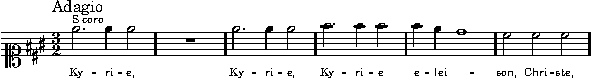
\includegraphics{incipits/2/1_regina}

  \item \textit{Sancta Virgo Virginum}\\\relax
    Adagio, A major, \metercut, 228 bars\\
    soli (2 S, A, T, B), coro (2 S, A, T, B), 2 vl, vlne, org\\
    \textlt{Kyrie eleison (19) · Mater Christi (86) · Rosa mystica (13) · Salus infirmorum (73) · Agnus Dei (37)}

    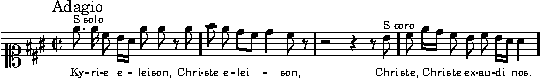
\includegraphics{incipits/2/2_sancta}

  \item \textit{Virgo clemens}\\\relax
    Adagio, B minor, \metercut, 224 bars\\
    soli (S, A, T, B), coro (S, A, T, B), 2 vl, vlne, org\\
    \textlt{Kyrie eleison (58) · Mater Creatoris (65) · Speculum iustitiae (70) · Agnus Dei (31)}

    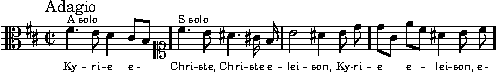
\includegraphics{incipits/2/3_virgo}

  \item \textit{Vas insigne devotionis}\\\relax
    Adagio, B minor, \metercut, 195 bars\\
    soli (S, A, T, B), coro (S, A, T, B), 2 vl, vlne, org\\
    \textlt{Kyrie eleison (51) · Virgo prudentissima (41) · Vas spirituale (66) · Agnus Dei (37)}

    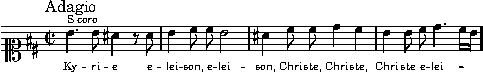
\includegraphics{incipits/2/4_vas}

  \item \textit{Causa nostrae laetitiae (longissimae)}\\\relax
    [no tempo], C dorian, \meterthreefour, 345 bars\\
    soli (S, A, T, B), coro (S, A, T, B), 2 vl, vlne, org\\
    \textlt{Kyrie eleison (67) · Sancta Maria (23) · Virgo prudentissima (84) · Rosa mystica (48) ·\\Regina Angelorum (37) · Agnus Dei (86)}

    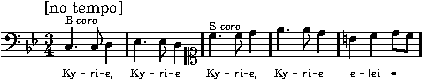
\includegraphics{incipits/2/5_causa}

  \item \textit{Sedes sapientiae}\\\relax
    Adagio, \sharp C\ minor, \meterthreetwo, 227 bars\\
    soli (S, A, T, B), coro (S, A, T, B), 2 vl, vlne, org\\
    \textlt{Kyrie eleison (66) · Sancta Maria (28) · Virgo prudentissima (64) · Foederis arca (35) · Agnus Dei (34)}

    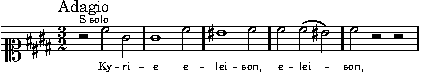
\includegraphics{incipits/2/6_sedes}

  \item \textit{Consolatrix afflictorum}\\\relax
    Adagio, D dorian, \metercut, 238 bars\\
    soli (S, A, T, B), coro (S, A, T, B), 2 vl, vlne, org\\
    \textlt{Kyrie eleison (7) · Pater de coelis (71) · Virgo prudentissima (23) · Rosa mystica (29) ·\\Salus infirmorum (42) · Agnus Dei (66)}

    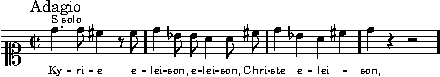
\includegraphics{incipits/2/7_consolatrix}

  \item \textit{Virgo prudentissima}\\\relax
    Adagio, D major, \meterthreetwo, 213 bars\\
    soli (S, A, T, B), coro (S, A, T, B), 2 vl, vlne, org\\
    \textlt{Kyrie eleison (80) · Sancta Maria (26) · Virgo prudentissima (57) · Rosa mystica (29) · Agnus Dei (21)}

    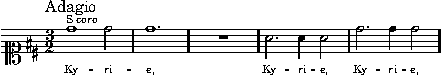
\includegraphics{incipits/2/8_virgo}

  \item \textit{Mater Christi}\\\relax
    [no tempo], E minor, \metercut, 239 bars\\
    soli (S, A, T, B), coro (S, A, T, B), 2 vl, vlne, org\\
    \textlt{Kyrie eleison (69) · Virgo prudentissima (94) · Salus infirmorum (18) · Regina Angelorum (25) ·\\Agnus Dei (33)}

    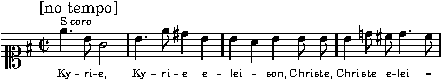
\includegraphics{incipits/2/9_mater}

  \item \textit{Mater purissima}\\\relax
    Adagio, F major, \metercut, 180 bars\\
    soli (S, A, T, B), coro (S, A, T, B), 2 vl, vlne, org\\
    \textlt{Kyrie eleison (32) · Mater amabilis (115) · Regina Angelorum (14) · Agnus Dei (19)}

    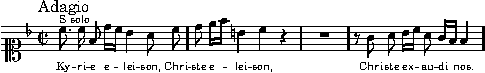
\includegraphics{incipits/2/10_mater}

  \item \textit{Stella matutina}\\\relax
    [no tempo], G dorian, \meterthreetwo, 253 bars\\
    soli (S, A, T, B), coro (S, A, T, B), 2 vl, vlne, org\\
    \textlt{Kyrie eleison (64) · Sancta Maria (39) · Speculum iustitiae (58) · Stella matutina (15) ·\\Regina Angelorum (17) · Agnus Dei (60)}

    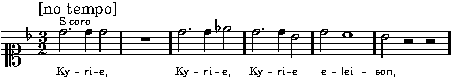
\includegraphics{incipits/2/11_stella}

  \item \textit{Rosa mystica}\\\relax
    Adagio, A minor, \metercommon, 180 bars\\
    soli (S, A, T, B), coro (S, A, T, B), 2 vl, vlne, org\\
    \textlt{Kyrie eleison (31) · Mater Creatoris (55) · Rosa mystica (51) · Agnus Dei (43)}

    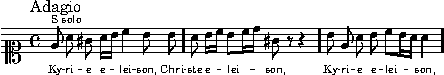
\includegraphics{incipits/2/12_rosa}
\end{enumerate}


\subsection{Sources}

\subsubsection{(1) Print}

\textsb{Classification}\\
notated music · print · copy · parts · fair copy · complete

\textsb{Locations}\\
A-Sd A 1502\\
D-B DMS 217257

\textsb{RISM}\\
990023743

\textsb{Publication, dating}\\
Johann Joseph Mayr, Salzburg, 1710

\pagebreak
\begin{flushleft}
  \textsb{Title page}\\
  \textit{[org part, fol. 1v]}\\
  \disablehyphenation CORONA | STELLARUM | DUODECIM. | ID EST | TOTIDEM | LITANIÆ | LAURETANO- | MARIANÆ, | SPECIALIBUS ENCOMIIS | MATRIS \& VIRGINIS | INTITULATÆ. | Partim à IV. partim à V. Vocibus, | \& II. Violinis in Concerto cum duplici Baſſo. | AUTHORE | MATTHÆO GUGL. | Anno à partu Virginis M.DCC.X. | in lucem datæ. | Opus I. ſumtibus Authoris. | ORGANO. | SALISBURGI, | Typis Joannis Joſephi Mayr, Typographi Aulico-Academici, \& Bibliopolæ.
\end{flushleft}

\vspace*{-\baselineskip}
The title pages of the remaining parts are mostly identical, with the exception of (1) the line “Opus I. …”, which only appears in the org part, and (2) the part name, which is replaced by one of “CANTUS I.”, “CANTUS II.” “ALTUS.”, “TENOR.”, “BASSUS.”, “VIOLINO I.”, or “VIOLINO II.”. Notably, an incorrect date (“M.DDC.X.”) is printed on the S~2 part. At the bottom, an ownership mark was written in brown ink by an unknown hand: “Ad Chorum Eccleſiæ SS. Trinitatis Salisburgi.” (the last word only appears on the title pages of the S~1 and org parts).


\textsb{Physical description}\\
9 parts\\
29.5 × 19 cm\\
up to 10 staves (10.5 mm)

\textsb{Components and notes}\\
The item in D-B consists of 8 parts (S 1, A, T, B, vl 1, vl 2, org (2x)) in a blue-brown marbled cardboard slipcase. The slipcase has two labels: one on the top left corner of the front side (“[printed:] Deutsche Musiksammlung | bei der Preußischen Staatsbibliothek, Berlin | Nr [in black pen:] 217257 1, (–8) | Gugl | [in pencil:] Cantus II fehlt”), and one on the spine (“DMS | 217257”). Each part (29.5 x 19 cm, up to 10 staves per page, staff size 10.5 mm) is bound in cardboard covered by the same blue-brown marbled paper as the slipcase and bears a label “LITANIÆ | MATTHÆI | GUGL. |”, followed by the part name “Cantus. I.|m|u|s”, “Altus.”, “Tenor.”, “Baſſus.”, “Violinum. I.|m|u|m”, “Violinum. II.”, or “Organo.”. A second label in the top left corner of the front cover contains the shelfmark “DMS | 217257”; below, an arabic numeral “1.” to “8.” has been written in black pen, numbering the parts.

The item in A-Sd comprises a single part (S~2; 29.5 x 19 cm, 9 staves per page, staff size 10.5 mm) bound in cardboard covered by blue-red-yellow marbled paper. Its cover label reads “LITANIÆ | MATTHÆI | GUGL. | Cantus. II.|d|u|s”. On the front inside cover, top left, the stamp reads: “Das Ahnenerbe | Außenſtelle Südoſt | Bücherei”, below it in pencil “X 334”; on the back inside cover, written vertically in pencil: “4 | S [lying down, =8?, =9?] | 1 [?] | S [lying down, =8?, =9?]”.

These two items form a complete set of parts. The paper contains the following watermarks: (1) GR [beneath coat of arms with Bavarian rhombs, crowned by mitre and crozier] / R; and (2) [savage man in cartouche (crowned, small)]. These watermarks indicate that the paper originates from two mills, namely (1) Georg Riepl, Raitenhaslach, Bavaria, and (2) Hofmann, Lengfelden.

The contents of the parts are as follows:

\begin{description}[labelwidth=1.5em,leftmargin=2em]
  \item[S 1] flyleaf, title page (fol. 1r), blank page (1v), music (2r–20v), contents (bottom of 20v), flyleaf.
  \item[S 2] flyleaf, title page (1r), blank page (1v), music (2r–4v), flyleaf. A note at the bottom of fol. 2v reads: “NB. | Cantus II. tantùm eſt in duabus primis Litaniis \textit{Regina Angelorum} \& \textit{Sancta Virgo} | \textit{Virginum}: In reliquis tantùm eſt I. Cantus.”.
  \item[A] flyleaf, title page (1r), blank page (1v), music (2r–20r), contents (20v), flyleaf.
  \item[T] flyleaf, title page (1r), blank page (1v), music (2r–18v), contents (bottom of 18v), flyleaf.
  \item[B] flyleaf, title page (1r), blank page (1v), music (2r–18r), contents (18v), flyleaf.
  \item[vl 1] flyleaf, title page (1r), blank page (1v), music (2r–17r), contents (17v), flyleaf.
  \item[vl 2] flyleaf, title page (1r), blank page (1v), music (2r–14v), contents (bottom of 14v), flyleaf.
  \item[org] Part “7.”: flyleaf, title page (1r; Figure~\ref{fig:corona_title}), blank page (1v), dedication and introduction (2r–3v), music (4r–24v; Figure~\ref{fig:corona_org}), contents (bottom of 24r; Figure~\ref{fig:corona_index}), flyleaf. Part “8.” lacks dedication and introduction; thus, music and contents appear on fol. 2r–22r and 22v, respectively.
\end{description}

\vspace*{-\baselineskip}
\begin{flushleft}
The \textsb{dedication and introduction} (org part, fol. 2r–3v) read:
\begin{description}[labelwidth=3em,leftmargin=3.5em]
  \item[fol. 2r] REVERENDISSIMO | AC | ILLUSTRISSIMO | DOMINO, DOMINO | MAXIMILIANO | ERNESTO, | COMITI AC DOMINO | A | SCHERFFENBERG, | Metropolit. Eccleſ. Salisburgenſis | PRÆPOSITO, | ET | ARCHI-PRESBYTERO. | PRÆPOSITO | Ad B. V. in Saal \& Isn. | Celſiſsimi ac Reverendiſsimi S.R.I.Prin- | cipis \& Archi-Epiſcopi Salisburgenſis. \&c. \&c. | CONSILIARIO INTIMO, | Nec non | Archi-Epiſcopalis Conſiſtorii ibidem | PRÆSIDI, \&c. | DOMINO DOMINO | GRATIOSISSIMO.
  \item[fol. 2v] REVERENDISSIME | AC ILLUSTRISSIME | DOMINE, DOMINE | COMES, | DOMINE DOMINE GRA- | TIOSISSIME, \&c. | FActum planè prodigioſum Sacra Scri- | ptura perhibet (a) dum \textit{duodecim} tribus Iſraël | ſuas in \textit{Tabernaculum fœderis} obtuliſſe Virgas | narrat. At ex his \textit{duodecim} unica tantùm Vir- | ga, quæ fuit \textit{tribûs Levi}, germinavit in Arcâ; | Eò quòd ſuper illam \textit{Aaronis} nomen ſignatum fuerit. | Reverendiſſime ac Illuſtriſſime Domine Domine Co- | mes \&c.\&c. \textit{Virgam egreſſam de radice Jeſſe} (b) \textit{Fœ-} | \textit{deris Arcam} Eccleſia, \& Gregorius Nicomedienſis (c) | \textit{Tabernaculum Domini} compellat. In hoc \textit{Tabernacu-} | \textit{lum} menti eſt mihi deferre faſciculum \textit{Virgarum Duode-} | \textit{cim}, nimirum haſce Litanias Lauretano·Parthenias, è qui- | bus \textit{Matri \& Virgini} coronam conflexi, quæ cum \textit{Stel-} | \textit{lam Jacob} reſpiciat, rectè \textit{Corona Stellarum Duodecim} (d) | nuncupari poteſt. At omnes iſtæ Virgulæ ſunt \textit{de Tribû} | \textit{Levi}, me videlicet Authore tam abjectò \& \textit{Levi}, ut non | abs re ſit hærere dubium, an in tam ſacra \textit{Tabernaculi} [footnote:] (a) \textit{Num.} 17.(b) \textit{Iſa.} 11. (c) \textit{Orat. de oblat.} (d) \textit{Apocal.} 12.
  \item[fol. 3r] Myſtici facie \textit{marceſcant} potiùs in faſtidiô, quàm \textit{germi-} | \textit{nent} in complacentiâ. Sed nova titubantem animum | confirmat anchora. Enim verò | \textit{Aaronem} in Te cerno, Reverendiſſime ac Illuſtriſſi- | me Domine, Domine Comes \&c.\&c. Nam velut Illum | Archi-Myſtam Iſraël, ſic Te Salipolis \textit{Archi-Presbyterum} | adorat. \textit{Aaronem} Te nominat, quidquid virtutum in | ullô Eccleſiæ Duce coruſcum fuit. Aaronem Te dicit | ipſa Nominis Ethymologia. (Quid enim \textit{Aaron} aliud apud | interpretes, quàm \textit{Mons} eſt?) Tu \textit{Mons} in \textit{parte} Nominis | \& quoad \textit{totum} omen \textit{Mons, in quô beneplacitum eſt Deo}. | (e) \textit{Aaronem} Te prædicat Sanctiſſima religio, Pietas \& Di- | lectio Dei ac hominum, præſertim Afflictorum. Qua- | rum Virtutum Laudes, ne hâc anguſtâ Paginâ contineri | poſſe videantur, potiùs cum fama miror, quàm venâ ri- | mor; Cùm aliàs etiam in tantâ materiæ copiâ illis, qui lau- | di ſunt impares, præſtet tenere ſilentium, quàm dixiſſe | nimis parum. Quapropter admitte, Reverendiſſime ac | Illuſtriſſime Domine, Domine Comes \&c.\&c. Admit- | te, ut Illuſtriſſimum Tuum (Veri \textit{Aaronis}) \textit{Nomen} ſig- | netur in hiſce meis \textit{duodecim} Virgultis. Tunc enim verò | uberes complacentiæ flores in Mariano \textit{Fœderis Taberna-} | \textit{culo} penitus germinatura confido. In quam me ſpem po- | tiſſimùm erigit, quòd fatô benigniſſimô ad \textit{B.V. in Saal} | primâ dignitate fulgeas. Placebit utique \textit{Deiparæ} Muſi- | ca, quam auſpicatur \textit{Præpoſitus} in Ejus \textit{aulâ}! Ego verò | \textit{immarceſcibili} ſtudiô laudabo Dominum \textit{in Chordis \&} | \textit{Organô}, (f) qui Te poſt longa adhuc \& Polycratæis fau- | ſtiora ſæcula tot jam pleniſſimum meritis \textit{Aaronem} indu- | cat \textit{in Sanctum Sanctorum}. (g) Cui voto immoritur, Tuís- | que ſe Gratiis ſubmiſſiſſimè commendat | Reverendiſsimæ ac Illuſtriſsimæ | Dominationis Tuæ | [in tiny print:] Servus humillimus | MATTHÆUS GUGL. [footnote:] (e) \textit{Pſal.} 67.(f) \textit{Pſal.} 150. (g) \textit{Num.} 4.
  \item[fol. 3v] \textit{Ad Philomuſum.} | VLtimum hujus quantulicúnque operis objectum | fuiſſe Hyperduliam Deiparæ, Te monitum volo; Cujus ſpe- | cialibus (ut mihi videbatur) Encomiis ſingulas inſcripſi Li- | tanias. Mens equidem fuit olim, pro ſingulis Lauretani | Catalogi Titulis ſingulas etiam Litanias ordinare: ſed interim perſuaſum | eſt, è tali copiâ plus vilipenſionis quàm uſurpationis oriturum. His | itáque Primitiis meis quædam notanda præpono. Primum eſt, quôd | labor iſte meus aliorum tantùm inſtinctû \& petitô in lucem datus ad | illos Choros, qui perfunctoriæ brevitati ſtudent, deſervire non poſſit: | Confido tamen, acceptum fore penitus, ubi plenus \& tarditatis Patiens | Chorus habetur. Favente autem Jehovâ opus aliud locis votísque plu- | ribus accomodatum typus vulgabit, \& congrua brevitas commendabit. | Alterum eſt, quòd huic opuſculo meo frequenter hoc ſignum \slashedsix\ inſertum | videatur \& idem valet, ac \sharp{}6. Iſte autem character \natural{}\ tonum natura- | lem indicat. Scio quidem, aliquas ex his Litaniis à me jam ante po- | ſtulatas \& deſcriptas fuiſſe: Sed eædem ipſæ priùs (quoad fieri potuit) | abbreviatæ, correctæ \& omni meliori modô emendatæ ſunt, antequam | typo crederentur. Errores admodum paucos ſuſcipor: Quos tamen | à Typographo inſertos reviſio mea, licet ſolertiſſima, non correxit, ſcien- | tia cujúsque Phonaſci eluet facillimè. Cæterùm hoc opuſculum meum | nondum ex totô impreſſum in varias jam cenſuras impegiſſe comperi. | Nimirum ſuis etiam Primitiæ fructuum roduntur vermibus. Tu, Ob- | ſervandiſſime Muſicophile, cum hisce Maſtygibus laborem hunc meum | maſticare omittes facilè, cum opus eſſe primum \& quidem ab Autho- | re juvene \& recente productum cogitaveris. Hoc igitur age, fave ac | vale.
\end{description}
\end{flushleft}


\subsubsection{(2) Manuscript copy}

\textsb{Classification}\\
notated music · manuscript · copy · parts · fair copy · excerpt

\textsb{Location}\\
D-OB MO 444

\textsb{RISM}\\
450007851

\textsb{Publication, dating}\\
ca. 1740

\textsb{Scribes}\\
unidentified (black ink)

\textsb{Title page}\\
\textit{[wrapper, fol. 1r]}\\
Lytaniæ Lauretanæ | à 4 Vocibus | Canto = Alto | Tenore \& Baſso | Con Organo \& | Violone | Authore Gugl.

\textsb{Physical description}\\
6 parts\\
36 × 21.5 cm\\
hand-ruled paper, 10 staves (10 mm)

\textsb{Components and notes}\\[1ex]
\begin{tabular}{ll}
  \toprule
  \itshape part & \itshape folios \\
  \midrule
  S solo and coro & 2 \\
  A solo and coro & 2 \\
  T solo and coro & 2 \\
  B solo and coro & 2 \\
  vlne            & 2 \\
  org             & 2 \\
  \bottomrule
\end{tabular}

Watermarks: (1) [coat of arms of Freiherr von Schönau] / ICF; and (2) [coat of arms of Freiherr von Schönau] / IMF. These watermarks indicate that the paper originates from the Ronsberg mill and was produced in ca.~1740 by Johann Carl Fischer or Johann Michael Fischer.

The manuscript contains an arrangement of the 8th litany (\textit{Virgo prudentissima}) for four voices and continuo, displaying the following differences:

\begin{tabularx}{\textwidth}{lllX}
  \toprule
  & \multicolumn{2}{l}{\itshape bars in source} \\
  \cmidrule{2-3}
  \itshape section & (1) & (2) & \itshape differences \\
  \midrule
  Kyrie eleison & 1–80 & 1–60 & 3/4 time; bars with vl solos removed (see Figure~\ref{fig:corona_intro}) \\
  Sancta Maria & 81–106 & 61–85 & almost identical (one bar removed) \\
  Virgo prudentissima & 107–163 & 86–136 & vl solos (bars 127–130 and 148–149) removed \\
  Rosa mystica & 164–192 & 137–165 & identical \\
  Agnus Dei & 193–213 & 166–186 & identical \\
  \bottomrule
\end{tabularx}



\clearpage
\section{GuglW 3: Missa Sanctissimae Trinitatis}

\textsb{Genre}\\
mass

\textsb{Scoring}\\
soli (S, A, T, B), coro (S, A, T, B), 2 clno, timp, 2 vl, 2 vla, vlne, org

\textsb{Place and date of composition}\\
Salzburg, 1712


\subsection{Music}

\begin{enumerate}
  \item \textit{Kyrie}\\\relax
    Adagio – Allegro, C major, \metercommon, 78 bars\\
    solo (S), coro (S, A, T, B), 2 clno, timp, 2 vl, 2 vla, vlne, org

    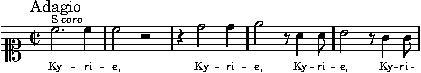
\includegraphics{incipits/3/1_kyrie}

  \item \textit{Gloria}\\\relax
    [no tempo], C major, \metercommon, 265 bars\\
    soli (S, A, T, B), coro (S, A, T, B), 2 clno, timp, 2 vl, 2 vla, vlne, org\\
    \textlt{Et in terra (24 bars) · Domine Deus (52) · Qui tollis (15) · Miserere (6) · Qui tollis (11) · \\
    Suscipe (20) · Qui sedes (15) · Miserere (11) · Quoniam (69) · Cum Sancto Spiritu (42)}

    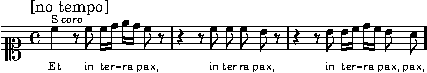
\includegraphics{incipits/3/2_gloria}

  \item \textit{Credo}\\\relax
    [no tempo], C major, \metercut, 296 bars\\
    soli (S, A, T, B), coro (S, A, T, B), 2 clno, timp, 2 vl, 2 vla, vlne, org\\
    \textlt{Patrem omnipotentem (14 bars) · Et in unum (77) · Qui propter (16) ·\\
    Et incarnatus est (13) · Crucifixus (19) · Passus (9) · Et resurrexit (34) ·\\
    Qui cum Patre (25) · Confiteor (41) · Et vitam (48)}

    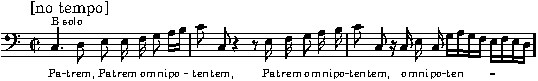
\includegraphics{incipits/3/3_credo}

  \pagebreak
  \item \textit{Sanctus}\\\relax
    [no tempo], C major, \meterthreefour, 113 bars\\
    soli (S, A, T), coro (S, A, T, B), 2 clno, timp, 2 vl, 2 vla, vlne, org\\
    \textlt{Sanctus (39 bars) · Pleni sunt coeli (49) · Osanna (25)}

    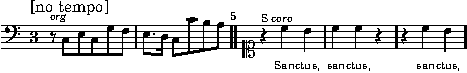
\includegraphics{incipits/3/4_sanctus}

  \item \textit{Benedictus}\\\relax
    [no tempo], C major, \meterthreefour, 68 bars\\
    soli (S, A, T), coro (S, A, T, B), 2 clno, timp, 2 vl, 2 vla, vlne, org\\
    \textlt{Benedictus (43 bars) · Osanna (25)}

    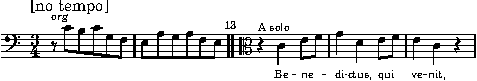
\includegraphics{incipits/3/5_benedictus}

  \item \textit{Agnus Dei}\\\relax
    [no tempo], C major, \metercommon, 103 bars\\
    soli (S, A, T, B), coro (S, A, T, B), 2 clno, timp, 2 vl, 2 vla, vlne, org\\
    \textlt{Agnus Dei (30 bars) · Osanna (73)}

    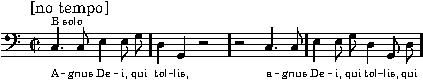
\includegraphics{incipits/3/6_agnus}
\end{enumerate}


\subsection{Sources}

\subsubsection{(1) Manuscript copy}

\textsb{Classification}\\
notated music · manuscript · copy · parts · fair copy · complete

\textsb{Location}\\
A-KR C 12/691

\textsb{RISM}\\
600172799

\textsb{Publication, dating}\\
1712

\textsb{Scribes}\\
unidentified (black ink)

\pagebreak
\textsb{Title page}\\
\textit{[wrapper, fol. 1r]}\\
Missa | SS|m|a|e Trinitatis | à | 4. Voci. | 2. Violini. | 2. Viole | 2. Clarini | Timpani | Organo con Violone | e | Basso per la Batutta. | L.H. | Auth. Matthaeo | Gugl. | 1712.

\textsb{Physical description}\\
14 parts\\
32 × 21 cm\\
hand-ruled paper, 10–11 staves (11 mm)

\textsb{Components and notes}\\[1ex]
\begin{tabular}{lll}
  \toprule
  \itshape part & \itshape folios & \itshape notes \\
  \midrule
  S solo and coro & 4 \\
  A solo and coro & 5 & Figure~\ref{fig:missa_alto} \\
  T solo and coro & 5 \\
  B solo and coro & 4 \\
  clno 1 & 2 \\
  clno 2 & 2 \\
  timp & 2 \\
  vl 1 & 4 & Figure~\ref{fig:missa_vl1} \\
  vl 2 & 4 \\
  vla 1 & 4 \\
  vla 2 & 4 \\
  vlne & 4 \\
  org & 6 & Figure~\ref{fig:missa_org} \\
  mdc & 6 \\
  \bottomrule
\end{tabular}


\clearpage
\section{GuglW 4: Quae est ista}

\textsb{Genre}\\
offertory

\textsb{Scoring}\\
solo (T), coro (S, A, T, B), 2 clno, timp, 2 vl, vlne, org

\textsb{Place and date of composition}\\
Salzburg, ca. 1710–20


\subsection{Music}

\begin{enumerate}
  \item \textit{Quae est ista}\\\relax
    Allegro, C major, \metercommon, 190 bars\\
    solo (T), coro (S, A, T, B), 2 clno, timp, 2 vl, 2 vla, vlne, org\\
    \textlt{Que est ista (27 bars) · Quae scandis aethera (58) · Exultate jubilate (105)}

    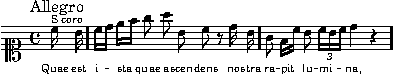
\includegraphics{incipits/4/1_quae}
\end{enumerate}


\subsection{Sources}

\subsubsection{(1) Manuscript copy}

\textsb{Classification}\\
notated music · manuscript · copy · parts · fair copy · complete

\textsb{Location}\\
A-LA 920

\textsb{RISM}\\
603001868

\textsb{Publication, dating}\\
1746–68

\textsb{Scribes}\\
Joseph Tischer (brown ink)

\textsb{Title page}\\
\textit{[wrapper, fol. 1r; see Figure~\ref{fig:quae_title}]}\\
Offertorium | Assumptione B:V:M: | a | Canto Alto. | Tenore Solo Basso. | Violinis 2bus | Clarinis 2bus | Tympano | con |Organo. | A.A.L. [= Amandus Abbas Lambacensis] | Descriptsit Josephus | Tischer | Del: Sig:|r|e Gugl

\textsb{Physical description}\\
10 parts\\
32 × 20.5 cm\\
hand-ruled paper, 10 staves (10 mm)

\textsb{Components and notes}\\[1ex]
\begin{tabular}{lll}
  \toprule
  \itshape part & \itshape folios & \itshape notes \\
  \midrule
  S coro & 2 & Figure~\ref{fig:quae_soprano}\\
  A coro & 2 \\
  T solo and coro & 2 \\
  B coro & 2 \\
  clno 1 & 1 \\
  clno 2 & 1 \\
  timp & 1 \\
  vl 1 & 2 \\
  vl 2 & 2 \\
  org & 2 & Figure~\ref{fig:quae_org} \\
  \bottomrule
\end{tabular}


\clearpage
\section{GuglW 5: Organ works}

\textsb{Genre}\\
preludes, versets, fugettas, miscellaneous

\textsb{Scoring}\\
org

\textsb{Place and date of composition}\\
Salzburg, ca. 1710–20


\subsection{Music}

This catalogue entry comprises all known organ works, which are numbered consecutively as GuglW~5.1 etc. (see first column in table below for the work subnumber).

Source (1) comprises the following works:

{\scriptsize
\begin{xltabular}{\textwidth}{>{\sbseries}r r r >{\raggedright}p{3cm} r m{6cm} X}
  \toprule
    &
    \itshape p. &
    \itshape no. &
    \itshape title &
    \itshape bars &
    \itshape incipit &
    \itshape notes \\
  \midrule
  \endhead
  \bottomrule
  \endfoot

  \tablesectionb{Primus tonus (D dorian), p. 1–9}
  1 & 1 & 1 & Gugl | Praeludium | 1mi Toni | ex D:m. del M: Gugl. & 7 & \includeincipit{1_1} & \\
  – & 1 & 2 & Caſpar Kerl. | Verſus 1. & 6 & \includeincipit{1_2} & attributed to Kerll \\
  2 & 1 & 3 & Verſus. 2. & 4 & \includeincipit{1_3} & \\
  3 & 2 & 1 & Verſus. 3. & 12 & \includeincipit{2_1} & \\
  4 & 2 & 2 & Verſus 4. & 10 & \includeincipit{2_2} & \\
  5 & 2 & 3 & Verſus 5. & 13 & \includeincipit{2_3} & bars 7–13 on p. 3\\
  6 & 3 & 1 & Finale. & 6 & \includeincipit{3_1} & \\
  7 & 3 & 2 & Verſus 6. & 7 & \includeincipit{3_2} & \\
  8 & 3 & 3 & Contra. [in pencil: 7] & 6 & \includeincipit{3_3} & \\
  9 & 4 & 1 & Verſus. [in pencil: 8] & 6 & \includeincipit{4_1} & \\
  10 & 4 & 2 & Verſus. [in pencil: 9] & 6 & \includeincipit{4_2} & \\
  11 & 4 & 3 & Verſus. [in pencil: 10] & 6 & \includeincipit{4_3} & \\
  12 & 4 & 4 & Verſus Contra.\newline [in pencil: 11] & 7 & \includeincipit{4_4} & \\
  – & 4 & 5 & Verſus. [in pencil: 12] & 4 & \includeincipit{4_5} & same as GuglW 5.2 \\
  13 & 5 & 1 & Verſus. [in pencil: 13] & 6 & \includeincipit{5_1} & \\
  14 & 5 & 2 & [in pencil: 14] & 5 & \includeincipit{5_2} & \\
  15 & 5 & 3 & Finale. & 3 & \includeincipit{5_3} & \\
  16 & 6 & 1 & Præludium. & 6 & \includeincipit{6_1} & \\
  17 & 6 & 2 & [in pencil: 15] & 4 & \includeincipit{6_2} & \\
  18 & 6 & 3 & [in pencil: 16] & 7 & \includeincipit{6_3} & \\
  19 & 7 & 1 & Verſus. [in pencil: 17] & 7 & \includeincipit{7_1} & \\
  20 & 7 & 2 & Gugl Verſ: [in pencil: 18] & 6 & \includeincipit{7_2} & \\
  21 & 7 & 3 & Verſ: [in pencil: 19] & 5 & \includeincipit{7_3} & \\
  22 & 8 & 1 & Verſus. [in pencil: 20] & 9 & \includeincipit{8_1} & \\
  23 & 8 & 2 & Verſ: [in pencil: 21] & 4 & \includeincipit{8_2} & \\
  24 & 8 & 3 & Verſ: Contra. & 3 & \includeincipit{8_3} & \\
  25 & 8 & 4 & Verſ: [in pencil: 23] & 5 & \includeincipit{8_4} & \\
  26 & 9 & 1 & Verſ: Contra [in pencil: 24] & 5 & \includeincipit{9_1} & \\
  27 & 9 & 2 & Verſ: [in pencil: 25] & 4 & \includeincipit{9_2} & \\
  28 & 9 & 3 & Verſus. [in pencil: 26] & 5 & \includeincipit{9_3} & \\
  29 & 9 & 4 & Præludium. & 7 & \includeincipit{9_4} & \\
  \midrule

  \tablesectionb{Secundus tonus (G dorian), p. 10–17}
  30 & 10 & 1 & Gugl Præludium 2:|d|i Toni. & 7 & \includeincipit{10_1} & \\
  31 & 10 & 2 & Verſus. & 6 & \includeincipit{10_2} & \\
  32 & 10 & 3 & Verſ. & 7 & \includeincipit{10_3} & \\
  33 & 11 & 1 & Verſus. & 18 & \includeincipit{11_1} & \\
  34 & 11 & 2 & Verſus. & 6 & \includeincipit{11_2} & \\
  35 & 12 & 1 & Gugl Præludi: & 5 & \includeincipit{12_1} & \\
  36 & 12 & 2 & [no title] & 7 & \includeincipit{12_2} & \\
  37 & 12 & 3 & Verſus. & 8 & \includeincipit{12_3} & \\
  38 & 13 & 1 & Verſ: & 6 & \includeincipit{13_1} & \\
  39 & 13 & 2 & [no title] & 8 & \includeincipit{13_2} & \\
  40 & 13 & 3 & Finale. & 5 & \includeincipit{13_3} & \\
  41 & 14 & 1 & Verſ: & 7 & \includeincipit{14_1} & \\
  42 & 14 & 2 & Verſ: & 6 & \includeincipit{14_2} & \\
  43 & 14 & 3 & Verſ: Contra. & 7 & \includeincipit{14_3} & \\
  44 & 15 & 1 & [no title] & 6 & \includeincipit{15_1} & \\
  45 & 15 & 2 & Verſus. & 11 & \includeincipit{15_2} & \\
  46 & 15 & 3 & Verſus. & 9 & \includeincipit{15_3} & \\
  47 & 16 & 1 & Verſ: & 6 & \includeincipit{16_1} & \\
  48 & 16 & 2 & Verſus. & 10 & \includeincipit{16_2} & \\
  49 & 17 & 1 & Verſ: & 8 & \includeincipit{17_1} & \\
  \midrule

  \tablesectionb{Tertius tonus (A aeolian), p. 18–23}
  50 & 18 & 1 & Præludium | 3.|t|i|j Toni | Gugl. & 11 & \includeincipit{18_1} & \\
  51 & 18 & 2 & Verſ & 8 & \includeincipit{18_2} & bars 5–8 on p. 19\\
  52 & 19 & 1 & Verſ & 8 & \includeincipit{19_1} & \\
  53 & 19 & 2 & Verſ: & 14 & \includeincipit{19_2} & \\
  54 & 20 & 1 & Præludium. | Gugl. & 5 & \includeincipit{20_1} & \\
  55 & 20 & 2 & [no title] & 24 & \includeincipit{20_2} & \\
  56 & 21 & 1 & Fugetta. & 28 & \includeincipit{21_1} & \\
  57 & 22 & 1 & Fugetta. & 17 & \includeincipit{22_1} & \\
  58 & 22 & 2 & Fugetta. & 23 & \includeincipit{22_2} & bars 15–23 on p. 23\\
  59 & 23 & 1 & Fugetta. & 8 & \includeincipit{23_1} & \\
  60 & 23 & 2 & Ultimo. & 11 & \includeincipit{23_2} & \\
  \midrule

  \tablesectionb{Quartus tonus (E phrygian), p. 24–31}
  61 & 24 & 1 & Præludium 4|t|i Toni. | Gugl & 6 & \includeincipit{24_1} & \\
  62 & 24 & 2 & Verſus. [in pencil: 1] & 4 & \includeincipit{24_2} & \\
  63 & 24 & 3 & Verſus. [in pencil: 2] & 7 & \includeincipit{24_3} & \\
  64 & 24 & 4 & Verſus. [in pencil: 3] & 5 & \includeincipit{24_4} & \\
  65 & 25 & 1 & [in pencil: 4] & 4 & \includeincipit{25_1} & \\
  66 & 25 & 2 & Finale. & 3 & \includeincipit{25_2} & \\
  67 & 25 & 3 & Verſus. [in pencil: 5] & 6 & \includeincipit{25_3} & \\
  68 & 25 & 4 & [in pencil: 6] & 6 & \includeincipit{25_4} & \\
  69 & 26 & 1 & Prælud: & 15 & \includeincipit{26_1} & \\
  70 & 27 & 1 & Fugetta. & 16 & \includeincipit{27_1} & \\
  71 & 27 & 2 & [in pencil: 7] & 4 & \includeincipit{27_2} & \\
  – & 28 & 1 & Verſus [in pencil: 8] & 6 & \includeincipit{28_1} & same as GuglW 5.68\\
  72 & 28 & 2 & Fugetta. & 13 & \includeincipit{28_2} & \\
  73 & 29 & 1 & Fugetta. & 27 & \includeincipit{29_1} & \\
  74 & 29 & 2 & [in pencil: 9] & 5 & \includeincipit{29_2} & \\
  75 & 30 & 1 & Verſus. [in pencil: 10] & 8 & \includeincipit{30_1} & \\
  76 & 30 & 2 & Verſus. [in pencil: 11] & 7 & \includeincipit{30_2} & \\
  77 & 30 & 3 & Verſus [in pencil: 12] & 5 & \includeincipit{30_3} & \\
  78 & 31 & 1 & Verſus [in pencil: 13] & 7 & \includeincipit{31_1} & \\
  \midrule

  \tablesectionb{Quintus tonus (C ionian), p. 32–37}
  79 & 32 & 1 & Præludium 5. Toni & 15 & \includeincipit{32_1} & \\
  80 & 32 & 2 & [no title] & 5 & \includeincipit{32_2} & \\
  81 & 33 & 1 & [no title] & 27 & \includeincipit{33_1} & \\
  82 & 33 & 2 & [no title] & 3 & \includeincipit{33_2} & \\
  83 & 34 & 1 & Fugetta. & 23 & \includeincipit{34_1} & \\
  84 & 34 & 2 & Verſus. & 13 & \includeincipit{34_2} & bars 9–13 on p. 35\\
  85 & 35 & 1 & Adagio. & 12 & \includeincipit{35_1} & \\
  86 & 36 & 1 & [no title] & 11 & \includeincipit{36_1} & \\
  87 & 36 & 2 & [no title] & 22 & \includeincipit{36_2} & bars 9–22 on p. 37\\
  \midrule

  \tablesectionb{Sextus tonus (F ionian), p. 38–44}
  88 & 38 & 1 & Præludium | 6.|t|i Toni & 11 & \includeincipit{38_1} & \\
  89 & 38 & 2 & Verſus. & 7 & \includeincipit{38_2} & \\
  90 & 39 & 1 & Verſus. & 6 & \includeincipit{39_1} & \\
  91 & 39 & 2 & [no title] & 7 & \includeincipit{39_2} & \\
  92 & 39 & 3 & [no title] & 18 & \includeincipit{39_3} & \\
  93 & 40 & 1 & Finale. & 4 & \includeincipit{40_1} & \\
  94 & 40 & 2 & Verſus. & 5 & \includeincipit{40_2} & \\
  95 & 40 & 3 & [no title] & 11 & \includeincipit{40_3} & \\
  96 & 41 & 1 & Verſus. & 16 & \includeincipit{41_1} & \\
  97 & 41 & 2 & Fugetta. & 14 & \includeincipit{41_2} & \\
  98 & 42 & 1 & Verſus. & 9 & \includeincipit{42_1} & \\
  99 & 42 & 2 & [no title] & 30 & \includeincipit{42_2} & bars 22–30 on p. 43\\
  100 & 43 & 1 & Verſus. & 16 & \includeincipit{43_1} & \\
  101 & 43 & 2 & Ultimo. & 7 & \includeincipit{43_2} & p. 44 empty\\
  \midrule

  \tablesectionb{Septimus tonus (D ionian), p. 45–48}
  102 & 45 & 1 & Præludium | 7:|m|i  Ton. & 5 & \includeincipit{45_1} & \\
  103 & 45 & 2 & [no title] & 8 & \includeincipit{45_2} & \\
  104 & 46 & 1 & [no title] & 24 & \includeincipit{46_1} & \\
  105 & 46 & 2 & [no title] & 7 & \includeincipit{46_2} & \\
  106 & 47 & 1 & [no title] & 10 & \includeincipit{47_1} & p. 48 empty\\
  \midrule

  \tablesectionb{Octavus tonus (G mixolydian), p. 49–56}
  107 & 49 & 1 & Præambul: | Octavi Toni & 13 & \includeincipit{49_1} & p. 49ff not paginated\\
  108 & 49 & 2 & [no title] & 7 & \includeincipit{49_2} & \\
  109 & 50 & 1 & [no title] & 15 & \includeincipit{50_1} & \\
  110 & 50 & 2 & [no title] & 8 & \includeincipit{50_2} & bars 5–8 on p. 51\\
  111 & 51 & 1 & [no title] & 11 & \includeincipit{51_1} & \\
  112 & 52 & 1 & Verſus. & 10 & \includeincipit{52_1} & \\
  113 & 52 & 2 & [no title] & 5 & \includeincipit{52_2} & \\
  – & 53 & 1 & [no title] & 13 & \includeincipit{53_1} & same as GuglW 5.107;\newline p. 54–56 empty\\
\end{xltabular}
}

Source (2) comprises one additional work and shares four works with source (1):

{\scriptsize
\begin{xltabular}{\textwidth}{>{\sbseries}r r r >{\raggedright}p{3cm} r m{6cm} X}
  \toprule
    &
    \itshape p. &
    \itshape no. &
    \itshape title &
    \itshape bars &
    \itshape incipit &
    \itshape notes \\
  \midrule
  \endhead
  \bottomrule
  \endfoot

  \tablesectionb{Quintus tonus (C ionian), p. 55–66}
  114 & 57 & 2 & Verſus | Del Sig. Gugl & 7 & \includeincipit{B_57_2} &  \\
  – & 60 & 1 & Fugetta | Del Sig: Gugl & 27 & \includeincipit{B_60_1} & same as GuglW 5.81 \\
  – & 61 & 1 & Fugetta | dal Sig: Gugl & 23 & \includeincipit{B_61_1} & same as GuglW 5.83 \\
  – & 62 & 1 & Fugetta | del Sig: Gugl & 13 & \includeincipit{B_62_1} & same as GuglW 5.84 \\
  – & 63 & 1 & Fugetta | Del Sig: Gugl & 11 & \includeincipit{B_63_1} & same as GuglW 5.86 \\
  \end{xltabular}
}


\subsection{Sources}

\subsubsection{(1) Manuscript copy}

\textsb{Classification}\\
notated music · manuscript · copy · score · fair copy · complete

\textsb{Location}\\
A-Ssp Gug 5.1

\textsb{RISM}\\
–

\textsb{Publication, dating}\\
ca. 1710–20

\textsb{Scribes}\\
unidentifed (black ink)

\textsb{Title page}\\
\textit{[wrapper, fol. 1r]}\\
Praeludia | et | Versus. | Del Sig: Mathaeo Gugl.

\textsb{Physical description}\\
1 score (28 fol.)\\
22 × 17.5 cm\\
hand-ruled paper, 10 staves (10 mm)

\textsb{Components and notes}\\[1ex]
see table above for details


\subsubsection{(2) Manuscript copy}

\textsb{Classification}\\
notated music · manuscript · copy · score · fair copy · complete

\textsb{Location}\\
D-Hs M A/801\\
(digitized version: \url{https://katalogplus.sub.uni-hamburg.de/vufind/Record/1969466030})

\textsb{RISM}\\
450035689

\textsb{Publication, dating}\\
ca. 1720–30

\textsb{Scribes}\\
Joseph Balthasar Hochreither (brown ink)

\textsb{Title page}\\
\textit{[fol. 1r]}\\\relax
[in pencil, by later hand; all brackets are reproduced from the source:] (J[oseph] B[althasar] Hochreitter, Schweighofer u. | [Matthäus] Gugl | Octitonium.) | [Anf. d. 18. Jhs.]

\pagebreak
\textsb{Physical description}\\
1 score (50 fol.)\\
17 × 24 cm\\
hand-ruled paper, 6 staves (10 mm)

\textsb{Components and notes}\\[1ex]
This source contains 159 organ works, of which 19 are attributed to Hochreither, 5 to Gugl, and 5 to (Severin) Schwaighofer. See \textcite{EsserSkala2026} for details and Figure~\ref{fig:octitonium}.

Watermarks: (1) R, in coat of arms with Bavarian rhombs, crowned by mitre and crozier [= no. 188 in the catalogue of A-Sd \parencite{Neumayr2018}; paper mill of Franz Anton Niederdorfer in Raitenhaslach]; and (2) savage man in cartouche (crowned, large) [= no. 25; paper mill of Johann Sigismund Hofmann, Lengfelden].



\begin{figure}[p]
  \centering
  \includegraphics[height=.95\textheight]{facsimile/corona_title}
  \caption{\textit{Corona stellarum duodecim}: Title page (fol. 1v) of the org part (D-B DMS 217257).}
  \label{fig:corona_title}
\end{figure}

\begin{figure}[p]
  \centering
  \includegraphics[height=.95\textheight]{facsimile/corona_org}
  \caption{\textit{Corona stellarum duodecim}: First page with music (fol. 4r) of the org part (D-B DMS 217257).}
  \label{fig:corona_org}
\end{figure}

\begin{figure}[p]
  \centering
  \includegraphics[height=.95\textheight]{facsimile/corona_index}
  \caption{\textit{Corona stellarum duodecim}: Table of contents (fol. 24r) of the org part (D-B DMS 217257).}
  \label{fig:corona_index}
\end{figure}

\begin{figure}[p]
  \centering
  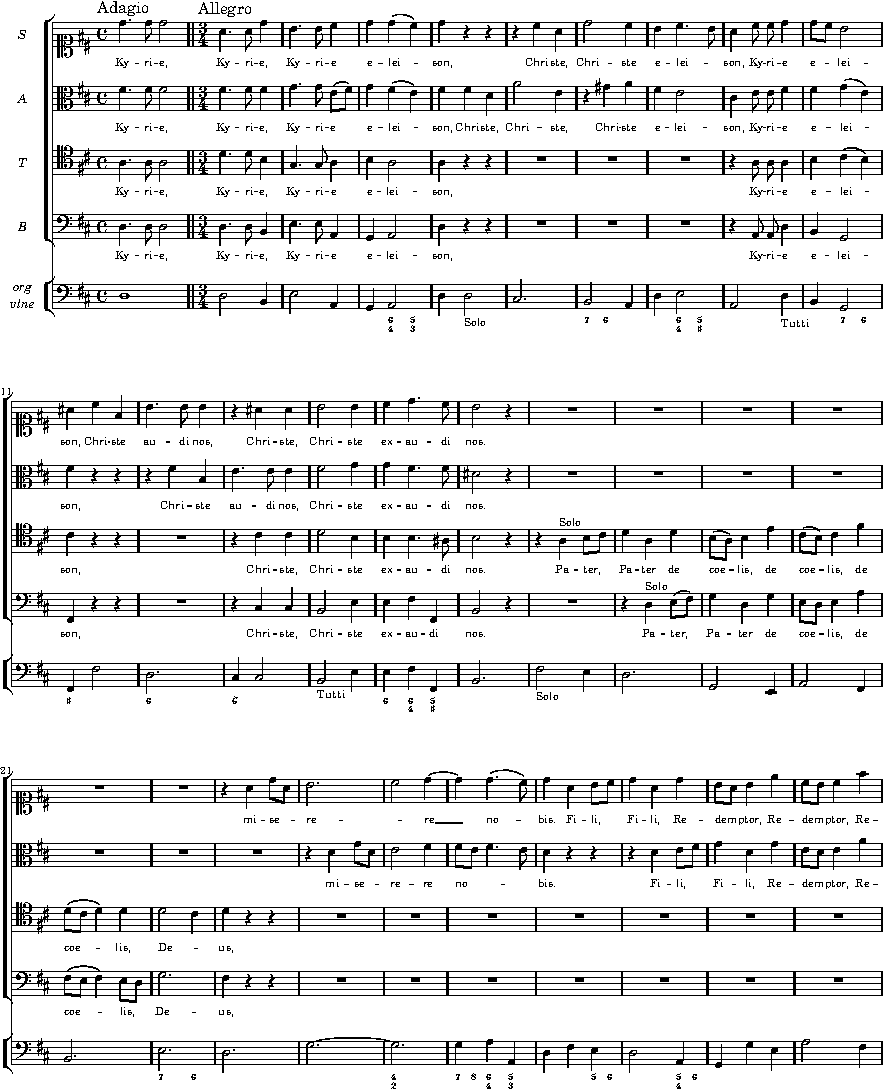
\includegraphics{corona_intro_1}
  \caption{\textit{Corona stellarum duodecim}: Alternative version of the section \textit{Kyrie eleison} in litany no.~8 (\textit{Virgo prudentissima}), which appears in the D-OB source (continued on next page).}
  \label{fig:corona_intro}
\end{figure}

\begin{figure}[p]
  \centering
  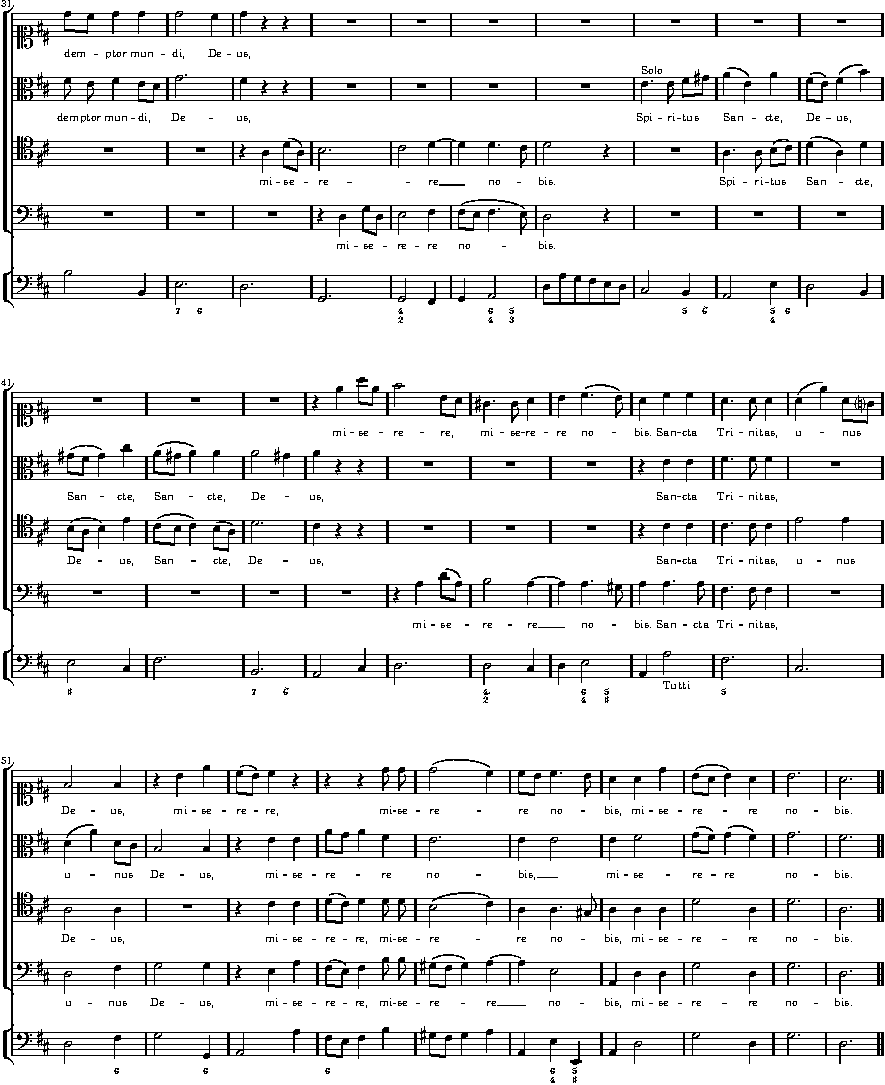
\includegraphics{corona_intro_2}
\end{figure}

\begin{figure}[p]
  \centering
  \includegraphics[height=.95\textheight]{facsimile/missa_alto}
  \caption{\textit{Missa Sanctissimae Trinitatis}: A part, fol. 1r (A-KR C 12/691).}
  \label{fig:missa_alto}
\end{figure}

\begin{figure}[p]
  \centering
  \includegraphics[height=.95\textheight]{facsimile/missa_vl1}
  \caption{\textit{Missa Sanctissimae Trinitatis}: vl 1 part, fol. 1r (A-KR C 12/691).}
  \label{fig:missa_vl1}
\end{figure}

\begin{figure}[p]
  \centering
  \includegraphics[height=.95\textheight]{facsimile/missa_org}
  \caption{\textit{Missa Sanctissimae Trinitatis}: org part, fol. 1r (A-KR C 12/691).}
  \label{fig:missa_org}
\end{figure}

\begin{figure}[p]
  \centering
  \includegraphics[height=.95\textheight]{facsimile/quae_title}
  \caption{\textit{Quae est ista}: wrapper, fol. 1r (A-LA 920).}
  \label{fig:quae_title}
\end{figure}

\begin{figure}[p]
  \centering
  \includegraphics[height=.95\textheight]{facsimile/quae_soprano}
  \caption{\textit{Quae est ista}: S part, fol. 1r (A-LA 920).}
  \label{fig:quae_soprano}
\end{figure}

\begin{figure}[p]
  \centering
  \includegraphics[height=.95\textheight]{facsimile/quae_org}
  \caption{\textit{Quae est ista}: org part, fol. 1r (A-LA 920).}
  \label{fig:quae_org}
\end{figure}

\begin{figure}[p]
  \centering
  \includegraphics[height=.90\textheight]{facsimile/octitonium}
  \caption{Two of Gugl's fugettas (GuglW 5.83 and 86) in the hand of Joseph Balthasar Hochreither (\textit{Octitonium}, D-Hs M A/801, p. 61 and 63).}
  \label{fig:octitonium}
\end{figure}


\cleardoublepage
\chapter{Critical report}

\section{Sources}

This edition bases upon the following principal sources (see catalogue of works for source descriptions):

\begin{tabularx}{\textwidth}{llX}
  \toprule
  \itshape work & \itshape source & \itshape location \\
  \midrule
  Corona stellarum duodecim     & \C1 & D-B DMS 217257 \\
                                & \C2 & A-Sd 1502 \\
  Missa Sanctissimae Trinitatis & \B1 & A-KR C 12/691 \\
  Quae est ista                 & \B1 & A-LA 920 \\
  \bottomrule
\end{tabularx}


\section{Commentary}

In general, this edition closely follows the principal source. Any changes that were introduced by the editor are indicated by italic type (lyrics, dynamics and directives), parentheses (expressive marks and bass figures) or dashes (slurs and ties). For further details, consult the Editorial Guidelines. Asterisks denote the following emendations:

\begin{xltabular}{\textwidth}{lll X}
  \toprule
  \itshape mov. & \itshape bar & \itshape staff & \itshape description \\
  \midrule \endhead
  \bottomrule \endfoot

  \tablesection{Corona stellarum duodecim}
  –  & –    & –    & The directives “S.” and “R.” in \C1/\C2 are reproduced as
                     “Solo” and “Tutti”, respectively. No additional dynamics
                     have been added. In the bass figures, “b” and \sharp{}\
                     are rendered as \natural{}\ if appropriate,
                     and \slashedsix\ is replaced by \natural6\ or
                     \doublesharp6. \sharp3\ and similar figures are reduced
                     to \sharp{}\ unless they indicate a single voice.
                     In \C1/\C2, double sharps are printed as single sharps,
                     but the modern convention is adopted here. \\
  1  & 31   & S 2  & bar in \C2: a′1. \\
     & 99   & S 2  & 2nd \quarterNote\ in \C2: \sharp c″4 \\
     & 182  & org  & 1st and 2nd \eighthNote\ of upper voice in \C1
                     indicated by bass figures \\
  2  & 88   & vl 1, A & 4th \quarterNote\ in \C1: d′4 \\
     & 119  & S 1  & time signature in \C1: 2/2 \\
     & 180  & A    & 1st \halfNote\ in \C1: d′2 \\
     & 221  & S 2  & 4th \eighthNote\ in \C2: \sharp g′8 \\
     & 210  & org  & 6th \eighthNote\ of upper voice in \C1
                     indicated by bass figures \\
     & 211  & org  & 3rd \quarterNote\ of upper voice in \C1
                     indicated by bass figures \\
  3  & 11   & S    & 1st \quarterNote\ in \C1: \sharp f″4 \\*
     & 12   & A    & 2nd \halfNote\ in \C1: \sharp f′4.–\sharp f′4 \\
     & 223  & A    & 1st \quarterNote\ in \C1: \sharp d′8 \\
  4  & 1    & A    & 1st to 3rd \quarterNote\ in \C1: \sharp f′4.–e′8–d′4 \\
     & 43f  & B    & voice added by editor \\
     & 137  & org  & last \eighthNote\ of upper voice in \C1
                     indicated by bass figures \\
     & 144  & org  & 4th \eighthNote\ of upper voice in \C1
                     indicated by bass figures \\
  5  & –    & org  & The directives “P.S.” (Basso solo, bar 42),
                     “T.S.” (Tenore solo, bars 117 and 181),
                     “W.” (Violini soli, bar 186), and
                     “B.S.” (Basso solo, bar 278) are omitted. \\
     & 77   & A    & 2nd \halfNote\ in \C1: e′4–\crotchetRest \\
     & 128  & org  & treble ottavo clef added by editor \\
     & 210  & A    & 2nd \halfNote\ in \C1: f′4–\quaverRest–g′8 \\
     & 237  & org  & 5th \eighthNote\ of upper voice in \C1
                     indicated by bass figures \\
     & 243  & org  & treble ottavo clef added by editor \\
     & 254  & org  & 5th \eighthNote\ of upper voice in \C1
                     indicated by bass figures \\
     & 257  & org  & 5th \eighthNote\ of upper voice in \C1
                     indicated by bass figures \\
     & 297ff & –   & “Solo” and “Tutti” in voices omitted \\
  6  & –    & org  & The directive “P.S.” (Basso solo, bar 86) is omitted. \\
     & 96   & org  & 3rd \quarterNote\ of upper voice in \C1
                     indicated by bass figures \\
     & 198  & A    & 3rd \eighthNote\ in \C1: \sharp g′8 \\
  7  & 27   & org  & 1st \quarterNote\ of upper voice in \C1
                     indicated by bass figures \\
     & 79   & vl 1, S, T & time signature in \C1: common time \\
     & 103f & org  & upper voice in \C1 indicated by bass figures \\
  8  & 15   & T    & 2nd \halfNote\ in \C1: \sharp c′2 \\
     & 104  & T    & 2nd \eighthNote\ in \C1: b8, corrected
                     with pencil to \sharp c′8 \\
  9  & –    & org  & The directive “C.S.” (Canto solo, bar 123) is omitted. \\
     & 31   & T    & 1st \quarterNoteDotted\ in \C1: b4. \\
     & 157  & vl 1 & 3rd \eighthNote\ in \C1: \sharp f″8 \\
     & 228f & org  & upper voice in \C1 indicated by bass figures \\
  10 & 4    & S, A & “Solo” and “Tutti” in voices omitted \\
     & 7    & vl 1 & 5th \eighthNote\ in \C2: \sharp f″8 \\
     & 8    & S    & 7th \eighthNote\ in \C1: e″8, corrected
                     with pencil to \sharp d″8 \\
     & 21   & T    & 2nd \quarterNote\ in \C1: c′4 \\
     & 65   & org  & upper voice in \C1 indicated by bass figures \\
     & 71   & S    & 3rd \quarterNote\ in \C1: a′4 \\
     & 106  & A    & “Tutti” in voice omitted \\
     & 173f & org  & upper voice in \C1 indicated by bass figures \\
  11 & –    & org  & The directives “Cant.S.” (Canto solo, bar 46)
                     and “A. S.” (Alto solo, bar 122) are omitted. \\
     & 92   & vl 1 & rhythm of 4th \eighthNote\ in \C1: 16.–32–32 \\
     & 101  & org  & treble ottavo clef added by editor \\
     & 249f & org  & treble ottavo clef added by editor \\
  12 & 7    & org  & upper voice in \C1 indicated by bass figures \\
     & 15   & org  & upper voice in \C1 indicated by bass figures \\
     & 87   & A, org & time signature in \C1: common time \\*
     & 89   & A    & 6th \eighthNote\ in \C1: \sharp f′8 \\
  \midrule

  \tablesection{Missa Sanctissimae Trinitatis}
  1 & 19   & S        & 1st \eighthNote\ in \B1: c″8 \\
    & 52   & clno 1   & last \eighthNote\ in \B1: f″8 \\
    & 53   & vlne     & bar in \B1: d4–e8–f8–g4–G4 \\
    & 65   & vla 2    & 1st \halfNote\ in \B1: g4–d′4 \\
    & 75   & vl 1     & bar in \B1: d″4–d″4–e″2 \\
  2 & 3    & vl 2     & 4th \sixteenthNote\ in \B1: g′16 \\
    & 102  & vla 1, A & 4th \halfNote\ in \B1: g′2 \\
    & 127f & timp     & bars in \B1: \wholeNoteRest and c1–c2 \\
    & 140  & A        & 4th \halfNote\ in \B1: g′2 \\
    & 148  & vla 1, A & 4th \halfNote\ in \B1: g′2 \\
    & 155  & clno 1   & 9th \eighthNote\ in \B1: g″8 \\
    & 189–199 & –     & It is unclear whether these bars should be performed
                        by soloists or chorus: In \B1, the directive “Tutti”
                        only appears in the S~part; vl~1/2 pause,
                        while~vla 1/2 play colla parte with A/T.
                        If this section is to performed by the chorus,
                        vl~1/2 may play colla parte with S,
                        as indicated by the notes in small print. \\
    & 210  & S        & 1st to 3rd \quarterNote\ in \B1: e″4–e″4–e″4 \\
    & 217  & B        & bar in \B1: A1–\halfNoteRest \\
    & 240ff & –       & From \B1, it is somewhat unclear which sections
                        should be performed by the chorus. This edition
                        shows only one of several possible variants. \\
    & 262  & vla 1    & 4th \quarterNote\ in \B1: g′8–g′8 \\
  3 & 82   & vla 1    & last \quarterNote\ in \B1: f′4 \\
    & 121–148 & –     & It is unclear whether these bars should be performed
                        by soloists or chorus: In \B1, there are neither “Solo”
                        nor “Tutti” directives; vl~1/2 pause,
                        while~vla 1/2 play colla parte with A/T.
                        If this section is to performed by the chorus,
                        vl~1/2 may play colla parte with S,
                        as indicated by the notes in small print. \\
    & 167  & vl 2     & 3rd \quarterNote\ in \B1: b′4 \\
    & 223  & vl 1     & bar missing in \B1 \\
    & 262  & clno 2   & bar in \B1: \wholeNoteRest \\
    & 270  & clno 2   & last \sixteenthNote\ in \B1: e″16 \\
    & 270f & timp     & 2nd \halfNote\ of bar 270 in \B1:
                        \quaverRest–c8–\quaverRest–c8;
                        1st \halfNote of bar 271: c8–c8-\crotchetRest \\
  4 & 13   & vl 1     & 3rd \quarterNote\ in \B1: d′′′8–d′′′8 \\
    & 33   & vla 2, T & bar in \B1: c′2. \\
    & 34   & clno 2   & 2nd \quarterNote\ in \B1: d″4 \\
    & 112  & vla 2    & 7th \eighthNote\ in \B1: b8 \\
  \midrule

  \tablesection{Quae est ista}
    & –   & –      & In \B1, the rhythm 16.–64–64 is written as 8.–32–32
                 (vl~1: bars 2, 8, 10, and 17; S: 10 and 17).
                 16th tuplets are always written as 8th tuplets
                 (S: bars 2 and 8). \\
    & 2   & clno 1 & 2nd \halfNote\ in \B1: d″4–\quaverRest–g″8 \\
    & 2   & timp   & 4th \quarterNote\ in \B1: \quaverRest–c8 \\
    & 2   & vl 2   & 14th to last \sixteenthNote\ in \B1: 3×e′16 \\
    & 2   & A      & 4th \eighthNote\ in \B1: e′8 \\
    & 5   & vl 2   & 4th \sixteenthNote\ in \B1: b′16 \\
    & 15  & A      & 15th \sixteenthNote\ in \B1: \sharp f′16 \\
    & 16  & T      & last \sixteenthNote\ in \B1: d′16 \\
    & 19  & T      & 7th \sixteenthNote\ in \B1: d′16 \\
    & 27  & vl 1   & 4th \quarterNote\ in \B1: c′4 \\
    & 29  & vl     & 4th \eighthNote\ in \B1: f′8 \\
    & 29  & org    & 1st \eighthNote\ in \B1: g8 \\
    & 62f & vl 2   & bars in \B1: c′4–d′4–c′4–d′8–c′8–d′4–c′4 and
                     b4–c′4–b4–c′2. \\
    & 67  & vl     & 1st \eighthNote\ in \B1: g8 \\
    & 72  & T      & 2nd \quarterNote\ in \B1: g′4 \\
    & 81  & vl 1   & rhythm of 4th \quarterNote\ in \B1: 16–16–8 \\
    & 89  & org    & 2nd \eighthNote\ in \B1: d8 \\
    & 108 & vl 2   & last \sixteenthNote\ in \B1: b′16 \\
    & 116 & B      & 7th \sixteenthNote\ in \B1: g16 \\
    & 128 & A      & 1st \quarterNote\ in \B1: c″4 \\
    & 141 & vl 2   & 4th \eighthNote\ in \B1: b′8 \\
    & 162 & org    & 2nd \eighthNote\ in \B1: B8 \\
    & 174 & timp   & bar missing in \B1 \\
    & 174 & org    & 2nd \eighthNote\ in \B1: c8 \\
    & 181 & vl 2   & 2nd \quarterNote\ in \B1: c″4 \\
    & 189 & vl 2   & 2nd \quarterNote\ in \B1: c″4 \\
\end{xltabular}
\setcounter{table}{0}



\subsection{Performance materials}

Performance materials for all works are available online under a Creative Commons Attribution-ShareAlike 4.0 International License, both on the edition's website via the given Archival Resource Keys (ARKs) and from the International Music Score Library Project (IMSLP). Moreover, the source code of all scores is available in LilyPond format from Codeberg.

\begin{tabular}{@{}ll}
  \multicolumn{2}{@{}l}{\itshape Corona Stellarum Duodecim} \\
  ARK   & \url{https://n2t.net/ark:68748/e1mgu2} \\
  IMSLP & \url{https://imslp.org/wiki/Category:Gugl%2C_Matth%C3%A4us} \\
  code  & \url{https://codeberg.org/edition-esser-skala/gugl-corona-stellarum-duodecim-GuglW-2} \\[1ex]
  \multicolumn{2}{@{}l}{\itshape Missa Sanctissimae Trinitatis} \\
  ARK   & \url{https://n2t.net/ark:68748/e1mgu3} \\
  IMSLP & \url{https://imslp.org/wiki/Category:Gugl%2C_Matth%C3%A4us} \\
  code  & \url{https://codeberg.org/edition-esser-skala/gugl-missa-sanctissimae-trinitatis-GuglW-3} \\[1ex]
  \multicolumn{2}{@{}l}{\itshape Quae est ista} \\
  ARK   & \url{https://n2t.net/ark:68748/e1mgu4} \\
  IMSLP & \url{https://imslp.org/wiki/Category:Gugl%2C_Matth%C3%A4us} \\
  code  & \url{https://codeberg.org/edition-esser-skala/gugl-quae-est-ista-GuglW-4} \\
\end{tabular}



\cleardoublepage
\chapter{Editorial guidelines}

(Below, we reproduce only the relevant excerpts from the \textit{Editorial Guidelines for the Edition Esser-Skala} v2026.01.0. The full version is available at \url{https://github.com/edition-esser-skala/ees-tools/blob/v2026.01.0/documents/editorial_guidelines.md}.)



\section*{Prefatory material}

\subsection{Critical report}

\paragraph{Sources}
This section describes the used sources of a given work. Each source is labeled with a bold capital letter (indicating the source category) followed by an index number:
\begin{bulletlist}
  \item \A{} – autograph manuscripts
  \item \B{} – other manuscripts used for the edition
  \item \C{} – prints used for the edition
  \item \D{} – manuscripts not used for the edition
  \item \E{} – prints not used for the edition
\end{bulletlist}

Within each category, sources are labeled in order of importance.

\paragraph{Commentary}
Each edition is based upon a single principal source, which is explicitly identified. Any substantial difference between the edition and the principal source is indicated with an asterisk in the score and reported in this section as an editorial \textit{emendation}.

However, the following elements are \textit{tacitly} modernized or standardized (see below for details): Tempo indications, instrument names, clefs, accidentals, beaming and stem directions, rests, placement of dynamics/slurs/ties, treatment of shorthand notations, bar numbering, bar lines, and repeats.

The table of emendations comprises the following columns:
\begin{bulletlist}
  \item movement (only if there are several movements in the work)
  \item bar number
  \item staff
  \item description
\end{bulletlist}

The following conventions apply to the commentary:
\begin{bulletlist}
  \item Keys are given with a capital letter for major or minor keys (e.g., “C minor”). Sharp and flat are spelled out with a hyphen (e.g., “B-flat major”).
  \item Notes are counted by ordinal numbers and written as symbol (e.g., “1st \quarterNote”).
  \item Helmholtz pitch notation is applied, with symbols for sharp, flat, and natural signs, and order name–accidental–octave (e.g., “\sharp c′”).
  \item Rests are written as symbol.
  \item A sequence of pitches is separated by en dashes (e.g., “c′4–d′8–e′8”)
  \item Chords are spelled with a plus sign between pitches from lowest to highest pitch (e.g., “c′+e′+g′4”).
  \item Modern English instrument names are used.
  \item Foreign words are typeset italic.
\end{bulletlist}


\section*{Conventions of notation}

\subsection{Score design}

The \textit{score order} from top to bottom is:
\begin{bulletlist}
  \item woodwind instruments (flutes, cornetts, oboes, chalumeaux, clarinets, bassoons)
  \item brass instruments (horns, trumpets, trombones)
  \item timpani
  \item strings (violins, violas, violoncellos, violones)
  \item voice parts (soprano, alto, tenor, bass)
  \item continuo
\end{bulletlist}

Families of instruments are barred and bracketed together. Voice parts are bracketed but barred separately. The continuo is bracketed. Pairs of instruments are either set in braces (e.g., violin I and II) or share one staff with automatic part combining. In the latter case,
\begin{bulletlist}
  \item polyphony may be indicated by opposing stems;
  \item the first and second parts get marked with their instrument abbreviations in solo situations; and
  \item the unison (a due) parts are marked with the text “a 2”.
\end{bulletlist}

Each part is spelled out in full on the first system of the first movement in the full score (singular form of modern Italian names); otherwise, it is abbreviated. Divided parts are indicated by Roman numerals in the first movement and by Arabic numbers in each subsequent movement. Transposing instruments include their pitch (e.g., “Clarino I, II in C” in the first movement and “clno (C) 1, 2” in subsequent movements). The part with figured bass is typically labeled “Organo e Bassi” or “Fondamento”.

In recitatives, instrumental parts also contain the solo vocal part. This convention typically applies to continuo parts in seccos and continuo plus string parts in accompagnatos.


\subsection{Clefs}

Keyboard music in soprano clef is notated in treble clef. Vocal music in soprano or alto clef is changed to treble clef; the tenor clef is changed to treble ottavo. Other clefs (e.g., alto for viola parts) are generally not altered. In the first movement, the original clef is given as incipit.


\subsection{Key signatures}

The original key signature is retained, while the order and position of sharps and flats is modernized.


\subsection{Tempo indications and movement designations}

Tempo indications appear in the original language; inconsistent spelling is regularized. Only the first word of Italian terms is capitalized (e.g., “Poco andante”). Movement designations may be retained in the original language (“Chor”) or translated to Italian (“Coro”). A missing tempo indication is denoted as “[no tempo]”.


Individual movements are numbered by the editor if numbers are absent in the source.


\subsection{Bar numbering}

Each new system except the first includes a bar number (bar 1 is the first full measure). Changes of tempo and meter within a movement are through-numbered. Bar numbering begins at 1 in each new movement, even where the movements are continuous (as indicated by thin-thin bar lines).


\subsection{Accidentals}

An accidental remains in force throughout a measure unless canceled by another accidental. Cautionary accidentals are tacitly added, redundant accidentals are tacitly deleted.


\subsection{Slurs and ties}

Slurs are carefully regularized. In vocal music, melismatic slurring in vocal music is shown even when beaming reflects syllabification. However, such slurs are usually not longer than one measure. Source slurring that shows phrasing is retained.

If two notes of the same pitch are tied, the note value is changed as appropriate.

Editorial slurs and ties are dashed.


\subsection{Bass figures}

Figures are set below the continuo line. Accidentals are placed before the figures to which they apply. Editorial figures are parenthesized. A resolution of the six-four chord like `6 4 → 3` is explicitly completed to `6 4 → [5] 3` or `6 4 → [7] 3` to avoid ambiguity with `6 4 → [6] 3`.


\subsection{Embellishments}

Ornaments are generally reproduced exactly as they appear in the principal source. Slurs are added from appoggiaturas to the main note, except if they appear under a longer slur. The rhythmic value of grace notes is tacitly emended to half the length of the main note. Editorial expressive marks are parenthesized.


\subsection{Articulation}

Generally, both dots and strokes in the source are rendered as strokes in the edition. Dots are only retained if they are required in a particular context such as portato (i.e., notes that are both slurred and dotted). Editorial articulation signs are parenthesized.


\subsection{Dynamics and directives}

Dynamics and other directives are usually standardized to modern Italian and placed below the staff, but above the staff in vocal music. Source dynamics are typeset upright, editorial additions or changes are typeset in italics.


\subsection{Notational shorthand}

Generally, notational shorthand is realized in full. Slashed stems may be used to indicate repeated notes if readability is improved.


\subsection{Vocal texts}

Latin texts are standardized and modernized. Archaic German spelling is retained (notably, lyrics distinguish between long ſ and round s). Editorial changes are indicated by italic type. When text is repeated in vocal music, a period is only used if a complete sentence is repeated; otherwise, a comma is used. Syllabification of German text is standardized according to the Duden. Groups of notes sung to a single syllable are beamed together, notes sung to separate syllables are stemmed separately.

\cleardoublepage%
\pagenumbering{arabic}%
\setcounter{page}{1}%
\includepdf[pages=-,link=true,linkname=score]{scores/2/full_score.pdf}%

\cleardoublepage
\includepdf[pages=-,link=true,linkname=score]{scores/3/full_score.pdf}%

\cleardoublepage
\includepdf[pages=-,link=true,linkname=score]{scores/4/full_score.pdf}%

\end{document}
